\documentclass[11pt]{report}

% --- Core Packages (order matters) ---
\usepackage[english]{babel}
\usepackage[utf8]{inputenc}
\usepackage[T1]{fontenc}

% --- Fonts ---
\usepackage[sfdefault]{roboto}        % Roboto as main font
\usepackage{sfmath}                    % Sans-serif math fonts for consistency
% Note: Using bold Roboto for headers instead of Roboto Slab (not in standard TeX Live)

% --- Graphics and Colors ---
\usepackage{graphicx}
\usepackage{xcolor}
\usepackage{tikz}
\usepackage{tikzpagenodes}

% --- Page Layout ---
\usepackage{geometry}
\geometry{a4paper, margin=2.5cm}

% --- Typography ---
\usepackage{microtype}
\setlength\parindent{0pt}
\setlength{\parskip}{1em}

\usepackage{pythontex}



% --- Section Formatting ---
\usepackage{titlesec}
\usepackage{sectsty}


% --- Figures and Tables ---
\usepackage{float}
\usepackage{caption}
\usepackage{subcaption}
\usepackage{booktabs}
\usepackage{multirow}

% --- Math ---
\usepackage{amsmath}
\usepackage{amssymb}

% --- Code Listings ---
\usepackage{listings}

% --- Bibliography ---
\usepackage[square,sort,comma,numbers]{natbib}

% --- Todo Notes ---
\usepackage[colorinlistoftodos]{todonotes}

% --- Title Customization ---
\usepackage{titling}
\usepackage{blindtext}

% --- Hyperlinks (load near end) ---
\usepackage{hyperref}

% --- TU Delft Colors ---
\definecolor{tudelftdarkblue}{RGB}{12,35,64}
\definecolor{tudelftcyan}{RGB}{0,166,214}
\definecolor{tudelftblue}{RGB}{0,118,194}

% --- Code Listing Colors ---
\definecolor{darkgreen}{rgb}{0.0, 0.4, 0.0}
\definecolor{codegreen}{rgb}{0,0.5,0.1}
\definecolor{codegray}{rgb}{0.5,0.5,0.5}
\definecolor{codepurple}{rgb}{0.58,0,0.67}
\definecolor{backcolour}{rgb}{0.92,0.94,0.96}
\definecolor{keywordcolor}{rgb}{0.8, 0.2, 0.4}

% --- Chapter and Section Styling ---
\titleformat{\chapter}[display]
  {\normalfont\huge\fontfamily{RobotoSlab-TLF}\bfseries\color{tudelftdarkblue}}
  {\chaptertitlename\ \thechapter}{20pt}{\Huge}

\titleformat{\section}
  {\normalfont\Large\fontfamily{RobotoSlab-TLF}\bfseries\color{tudelftdarkblue}}
  {\thesection}{1em}{}

\titleformat{\subsection}
  {\normalfont\large\fontfamily{RobotoSlab-TLF}\bfseries\color{tudelftdarkblue}}
  {\thesubsection}{1em}{}

\titleformat{\subsubsection}
  {\normalfont\normalsize\fontfamily{RobotoSlab-TLF}\bfseries\color{tudelftblue}}
  {\thesubsubsection}{1em}{}

% --- Hyperlink Setup ---
\hypersetup{
  colorlinks=true,
  linkcolor=tudelftblue,
  urlcolor=tudelftblue,
  citecolor=tudelftblue,
  bookmarksdepth=3,
  pdfauthor={Alessandro Valmori},
  pdftitle={Machine and Deep Learning - Lecture Notes}
}

% --- Caption Styling ---
\captionsetup{
  font=small,
  labelfont={bf,color=tudelftdarkblue},
  textfont=it
}

% --- Code Listing Style ---
\lstdefinestyle{mystyle}{
  backgroundcolor=\color{backcolour},
  commentstyle=\color{codegreen}\itshape,
  keywordstyle=\color{keywordcolor}\bfseries,
  numberstyle=\tiny\color{codegray},
  stringstyle=\color{codepurple},
  basicstyle=\ttfamily\footnotesize,
  breakatwhitespace=false,
  breaklines=true,
  captionpos=b,
  keepspaces=true,
  numbers=left,
  numbersep=5pt,
  showspaces=false,
  showstringspaces=false,
  showtabs=false,
  tabsize=2,
  frame=single,
  rulecolor=\color{codegray!30}
}
\lstset{style=mystyle}

%%%%%%%%%%%%%%%%%%%%%%%%%%%%%%%%%%%%%%%%%%%%%%%%%%%%%%%%%
\begin{document}

\begin{pycode}
import sys
import os
import numpy as np
import matplotlib.pyplot as plt

# Ensure pythontex looks in the current directory for plot_utils.py
sys.path.append(os.getcwd())

# Import our custom module
import plot_utils as utils

# Apply the global style immediately
utils.set_style()
\end{pycode}

% --- Custom Title Page ---
\begin{titlepage}
	\fontfamily{RobotoSlab-TLF}\selectfont
	\centering
	\vspace*{3cm}

	{\Huge\bfseries\color{black} Lecture Notes}\\[1.5cm]

	{\LARGE\scshape Machine Learning}\\[0.5cm]

	{\large DSAIT4005}\\[3cm]

	{\Large\bfseries\color{tudelftdarkblue} Author}\\[0.5cm]

	{\Large\color{tudelftdarkblue} Alessandro Valmori}\\[3cm]

	{\Large\color{tudelftdarkblue}\today}

	\vfill

	\includegraphics[width=0.6\textwidth]{images/TU_delft_logo.jpg}

	\vspace{1cm}
\end{titlepage}

\tableofcontents
\newpage

%--- CHAPTER 1: Machine Learning ---
\chapter{Machine Learning}
\label{chap:ml}

\section{Classification}
\label{sec:ml_classification}
% In your machine_learning.tex file, under \section{Classification}

The primary goal of a classification task is to assign a class label, $y$, to an object represented by a feature vector, $\mathbf{x}$. A robust way to achieve this is by estimating the \textbf{posterior probability}, denoted as $p(y|\mathbf{x})$. This value represents the probability that a given object $\mathbf{x}$ belongs to class $y$. The class with the highest posterior probability is then chosen as the prediction.

\subsection{Generative Classification via Bayes' Theorem}
Directly estimating the posterior probability can be challenging. An alternative is to use a \textbf{generative approach}, which models the underlying probability distributions of the data. The core of this method is \textbf{Bayes' theorem}, which elegantly connects the posterior probability to other, more manageable components:

\begin{equation}
	p(y|\mathbf{x}) = \frac{p(\mathbf{x}|y)p(y)}{p(\mathbf{x})}
	\label{eq:bayes_theorem}
\end{equation}

Each term in this equation has a distinct and important role:
\begin{itemize}
	\item \textbf{$p(y|\mathbf{x})$ (Posterior Probability):} This is what we aim to compute. It's the probability of a class label $y$ \textit{after} observing the data $\mathbf{x}$.

	\item \textbf{$p(\mathbf{x}|y)$ (Likelihood or Class-Conditional Density):} This is the probability of observing the data point $\mathbf{x}$ given that it belongs to class $y$. We often make assumptions about this distribution, for example, that the data for each class follows a Gaussian distribution.

	\item \textbf{$p(y)$ (Prior Probability):} This is the probability of class $y$ occurring, independent of the data. It reflects our prior belief about how common each class is. For instance, if we know a dataset contains 70\% cats and 30\% dogs, these would be our priors.

	\item \textbf{$p(\mathbf{x})$ (Evidence or Marginal Likelihood):} This is the overall probability of observing the data point $\mathbf{x}$ across all classes. It acts as a normalization constant to ensure that the posterior probabilities sum to 1. It can be calculated by summing over all classes $y_i$: $p(\mathbf{x}) = \sum_{i} p(\mathbf{x}|y_i)p(y_i)$.
\end{itemize}

This approach is called ``generative'' because by modeling the likelihood $p(\mathbf{x}|y)$ and the prior $p(y)$, we are effectively learning a model of how the data for each class is generated.

\subsection{Bayes' Decision Rule and Conditional Risk}
\label{sec:ml_conditional_risk}
While choosing the class with the maximum posterior probability $p(y|\mathbf{x})$ is often the default, it implicitly assumes that all misclassifications have an equal cost. In many real-world scenarios, this is not true. For example, in medical diagnosis, misclassifying an 'ill' patient as 'healthy' can be far more dangerous and costly than misclassifying a 'healthy' patient as 'ill'.

To handle this, we introduce a \textbf{loss matrix} (or cost function), $\lambda$, where $\lambda_{ji}$ represents the cost or loss incurred for assigning an object to class $y_i$ when its true class is $y_j$.

Our goal shifts from simply maximizing probability to minimizing the expected loss. We can quantify this expected loss for a given observation $\mathbf{x}$ by defining the \textbf{conditional risk} $l^i(\mathbf{x})$ associated with deciding for class $y_i$:

\begin{equation}
	l^i(\mathbf{x}) = \sum_{j=1}^{C} \lambda_{ji} p(y_j|\mathbf{x})
	\label{eq:conditional_risk}
\end{equation}

The conditional risk $l^i(\mathbf{x})$ is the expected loss of choosing class $y_i$. It is a weighted sum over all possible \textit{true} classes $y_j$. For each $y_j$, we multiply the cost of our decision ($\lambda_{ji}$) by the posterior probability that $y_j$ is the true class ($p(y_j|\mathbf{x})$).

The \textbf{Bayes' decision rule} is to choose the class $y_i$ that \textbf{minimizes the conditional risk}:
\begin{itemize}
	\item Assign $\mathbf{x}$ to class $y_i$ if $l^i(\mathbf{x}) \le l^k(\mathbf{x})$ for all $k=1, \dots, C$.
\end{itemize}

\subsubsection{The 0-1 Loss Function}
The standard maximum posterior rule is a special case of this framework. It corresponds to a \textbf{0-1 loss function}, where:
\begin{itemize}
	\item $\lambda_{ji} = 0$ if $i = j$ (correct decision, zero cost)
	\item $\lambda_{ji} = 1$ if $i \ne j$ (any error, unit cost)
\end{itemize}
In this case, the conditional risk for choosing $y_i$ becomes:
$$
	l^i(\mathbf{x}) = \sum_{j \ne i} (1) \cdot p(y_j|\mathbf{x}) + (0) \cdot p(y_i|\mathbf{x}) = \sum_{j \ne i} p(y_j|\mathbf{x})
$$
Since $\sum_{j=1}^{C} p(y_j|\mathbf{x}) = 1$, we can rewrite this as $l^i(\mathbf{x}) = 1 - p(y_i|\mathbf{x})$. Minimizing $1 - p(y_i|\mathbf{x})$ is mathematically identical to maximizing $p(y_i|\mathbf{x})$.

\subsubsection{Two-Class Example}
For a two-class problem ($y_1, y_2$), assuming $\lambda_{11} = \lambda_{22} = 0$ (no cost for correct classification), we compare the risks:
\begin{itemize}
	\item Risk of choosing $y_1$: $l^1(\mathbf{x}) = \lambda_{11}p(y_1|\mathbf{x}) + \lambda_{21}p(y_2|\mathbf{x}) = \lambda_{21}p(y_2|\mathbf{x})$
	\item Risk of choosing $y_2$: $l^2(\mathbf{x}) = \lambda_{12}p(y_1|\mathbf{x}) + \lambda_{22}p(y_2|\mathbf{x}) = \lambda_{12}p(y_1|\mathbf{x})$
\end{itemize}
The minimum risk rule is to choose $y_1$ if $l^1(\mathbf{x}) \le l^2(\mathbf{x})$, which simplifies to:
\begin{equation}
	\lambda_{21}p(y_2|\mathbf{x}) \le \lambda_{12}p(y_1|\mathbf{x})
\end{equation}
This decision rule directly incorporates the asymmetric costs, effectively "pushing" the decision boundary away from the class with the higher misclassification cost.


\subsection{The Gaussian Plug-in Approach}
The "plug-in" approach involves estimating the components of Bayes' theorem (Equation \ref{eq:bayes_theorem}) from the training data. For a given class $y_i$, we need to estimate:
\begin{enumerate}
	\item \textbf{The Prior Probability $\hat{p}(y_i)$:} This is typically estimated as the fraction of training samples belonging to that class. If $N_i$ is the number of samples in class $y_i$ and $N$ is the total number of samples, then:
	      \begin{equation}
		      \hat{p}(y_i) = \frac{N_i}{N}
	      \end{equation}

	\item \textbf{The Class-Conditional Probability $\hat{p}(\mathbf{x}|y_i)$:} This is the most critical modeling choice. We assume that the data for each class follows a \textbf{multivariate Gaussian distribution}. This distribution is defined by a mean vector $\boldsymbol{\mu}$ and a covariance matrix $\boldsymbol{\Sigma}$.
\end{enumerate}

The probability density function for a $d$-dimensional multivariate Gaussian distribution is given by:
\begin{equation}
	p(\mathbf{x} | \boldsymbol{\mu}, \boldsymbol{\Sigma}) = \frac{1}{\sqrt{(2\pi)^d \det(\boldsymbol{\Sigma})}} \exp\left(-\frac{1}{2}(\mathbf{x}-\boldsymbol{\mu})^T \boldsymbol{\Sigma}^{-1} (\mathbf{x}-\boldsymbol{\mu})\right)
	\label{eq:multivariate_gaussian}
\end{equation}
Where:
\begin{itemize}
	\item $\boldsymbol{\mu}$ is the $d$-dimensional mean vector, which defines the center of the distribution.
	\item $\boldsymbol{\Sigma}$ is the $d \times d$ covariance matrix, which describes the shape and orientation of the distribution's contour. The diagonal elements contain the variances of each feature, and the off-diagonal elements contain the covariances between features.
\end{itemize}

To use this model, we must estimate a separate mean $\boldsymbol{\hat{\mu}}_i$ and covariance matrix $\boldsymbol{\hat{\Sigma}}_i$ for each class $y_i$. We can do this using the training data for that class, typically with Maximum Likelihood Estimators:
\begin{align}
	\boldsymbol{\hat{\mu}}_i    & = \frac{1}{N_i} \sum_{\mathbf{x}_k \in \text{class } y_i} \mathbf{x}_k \label{eq:mle_mean}                                                                               \\
	\boldsymbol{\hat{\Sigma}}_i & = \frac{1}{N_i} \sum_{\mathbf{x}_k \in \text{class } y_i} (\mathbf{x}_k - \boldsymbol{\hat{\mu}}_i)(\mathbf{x}_k - \boldsymbol{\hat{\mu}}_i)^T \label{eq:mle_covariance}
\end{align}

By plugging these estimated Gaussian distributions into Bayes' theorem, we create a powerful classification model.


\subsection{Quadratic Discriminant Classifier (QDA)}
Our decision rule is to assign a feature vector $\mathbf{x}$ to the class $y_i$ that maximizes the posterior probability $p(y_i|\mathbf{x})$. Because the logarithm is a monotonically increasing function, maximizing $p(y_i|\mathbf{x})$ is equivalent to maximizing $\log(p(y_i|\mathbf{x}))$. This allows us to define a \textbf{discriminant function} $g_i(\mathbf{x})$ for each class:

\begin{equation}
	g_i(\mathbf{x}) = \log(p(y_i|\mathbf{x})) = \log(p(\mathbf{x}|y_i)) + \log(p(y_i)) - \log(p(\mathbf{x}))
\end{equation}

Since we are only interested in which class has the largest value, we can drop the term $\log(p(\mathbf{x}))$ because it is the same for all classes and does not affect the final decision.

Now, we substitute the multivariate Gaussian formula (Equation \ref{eq:multivariate_gaussian}) into the likelihood term $\log(p(\mathbf{x}|y_i))$:
\begin{align}
	g_i(\mathbf{x}) & \propto \log\left( \frac{1}{\sqrt{(2\pi)^d \det(\boldsymbol{\Sigma_i})}} \exp\left(-\frac{1}{2}(\mathbf{x}-\boldsymbol{\mu_i})^T \boldsymbol{\Sigma_i}^{-1} (\mathbf{x}-\boldsymbol{\mu_i})\right) \right) + \log(p(y_i)) \nonumber \\
	                & = -\frac{1}{2}\log\left((2\pi)^d \det(\boldsymbol{\Sigma_i})\right) - \frac{1}{2}(\mathbf{x}-\boldsymbol{\mu_i})^T \boldsymbol{\Sigma_i}^{-1} (\mathbf{x}-\boldsymbol{\mu_i}) + \log(p(y_i))
\end{align}

Again, we can drop the constant term $-\frac{1}{2}\log((2\pi)^d)$ as it's the same for all classes. This leaves us with the final form of the discriminant function for QDA:
\begin{equation}
	g_i(\mathbf{x}) = -\frac{1}{2}(\mathbf{x}-\boldsymbol{\mu_i})^T \boldsymbol{\Sigma_i}^{-1} (\mathbf{x}-\boldsymbol{\mu_i}) - \frac{1}{2}\log(\det(\boldsymbol{\Sigma_i})) + \log(p(y_i))
	\label{eq:qda_discriminant}
\end{equation}

\subsubsection{Deconstructing the QDA Discriminant Function}
Let's analyze the three components of $g_i(\mathbf{x})$:
\begin{enumerate}
	\item \textbf{$-\frac{1}{2}(\mathbf{x}-\boldsymbol{\mu_i})^T \boldsymbol{\Sigma_i}^{-1} (\mathbf{x}-\boldsymbol{\mu_i})$:} This is the core quadratic term. The expression $(\mathbf{x}-\boldsymbol{\mu_i})^T \boldsymbol{\Sigma_i}^{-1} (\mathbf{x}-\boldsymbol{\mu_i})$ is the squared \textbf{Mahalanobis distance}. It measures the distance from the point $\mathbf{x}$ to the class mean $\boldsymbol{\mu_i}$, "scaled" by the class covariance $\boldsymbol{\Sigma_i}$. This term is large and negative if $\mathbf{x}$ is far from the mean $\boldsymbol{\mu_i}$ (relative to the class-specific covariance), thus penalizing the score for that class.

	\item \textbf{$-\frac{1}{2}\log(\det(\boldsymbol{\Sigma_i}))$:} This term depends only on the determinant of the class covariance matrix. The determinant, $\det(\boldsymbol{\Sigma_i})$, is a measure of the "volume" or "spread" of the data in class $i$. A class with a larger, more spread-out distribution (larger determinant) receives a penalty to its score. This makes intuitive sense: a point is "less surprisingly" near a spread-out distribution, so the model requires more evidence to assign it to that class.

	\item \textbf{$\log(p(y_i))$:} This is the log of the prior probability. It shifts the entire discriminant function for class $i$ up or down. If a class $i$ is very common (high prior), its score gets a boost, making the model more likely to choose it, all else being equal.
\end{enumerate}

\subsubsection{The Quadratic Decision Boundary}
The decision boundary between two classes, $y_i$ and $y_j$, is the set of all points $\mathbf{x}$ where the discriminant scores are equal: $g_i(\mathbf{x}) = g_j(\mathbf{x})$.

Let's look more closely at the quadratic term. We can expand the full discriminant function (Equation \ref{eq:qda_discriminant}) into its general polynomial form:
\begin{align}
	g_i(\mathbf{x}) & = -\frac{1}{2} (\mathbf{x}^T \boldsymbol{\Sigma_i}^{-1} \mathbf{x} - \mathbf{x}^T \boldsymbol{\Sigma_i}^{-1} \boldsymbol{\mu_i} - \boldsymbol{\mu_i}^T \boldsymbol{\Sigma_i}^{-1} \mathbf{x} + \boldsymbol{\mu_i}^T \boldsymbol{\Sigma_i}^{-1} \boldsymbol{\mu_i}) - \frac{1}{2}\log(\det(\boldsymbol{\Sigma_i})) + \log(p(y_i)) \nonumber \\
	                & = -\frac{1}{2} \mathbf{x}^T \boldsymbol{\Sigma_i}^{-1} \mathbf{x} + \mathbf{x}^T (\boldsymbol{\Sigma_i}^{-1} \boldsymbol{\mu_i}) + \left( -\frac{1}{2} \boldsymbol{\mu_i}^T \boldsymbol{\Sigma_i}^{-1} \boldsymbol{\mu_i} - \frac{1}{2}\log(\det(\boldsymbol{\Sigma_i})) + \log(p(y_i)) \right)
\end{align}
Note that $\mathbf{x}^T \boldsymbol{\Sigma_i}^{-1} \boldsymbol{\mu_i}$ is a scalar, and since $\boldsymbol{\Sigma_i}^{-1}$ is symmetric, it is equal to $\boldsymbol{\mu_i}^T \boldsymbol{\Sigma_i}^{-1} \mathbf{x}$.

This simplifies to the general quadratic form $g_i(\mathbf{x}) = \mathbf{x}^T \mathbf{A}_i \mathbf{x} + \mathbf{b}_i^T \mathbf{x} + c_i$, where:
\begin{itemize}
	\item $\mathbf{A}_i = -\frac{1}{2} \boldsymbol{\Sigma_i}^{-1}$ (a matrix, hence the $\mathbf{x}^T \dots \mathbf{x}$ term)
	\item $\mathbf{b}_i = \boldsymbol{\Sigma_i}^{-1} \boldsymbol{\mu_i}$ (a vector, hence the $\dots^T \mathbf{x}$ term)
	\item $c_i = -\frac{1}{2} \boldsymbol{\mu_i}^T \boldsymbol{\Sigma_i}^{-1} \boldsymbol{\mu_i} - \frac{1}{2}\log(\det(\boldsymbol{\Sigma_i})) + \log(p(y_i))$ (a scalar constant)
\end{itemize}

The decision boundary $g_i(\mathbf{x}) - g_j(\mathbf{x}) = 0$ is therefore defined by the equation:
\begin{equation}
	\mathbf{x}^T (\mathbf{A}_i - \mathbf{A}_j) \mathbf{x} + (\mathbf{b}_i - \mathbf{b}_j)^T \mathbf{x} + (c_i - c_j) = 0
	\label{eq:qda_boundary}
\end{equation}

Crucially, in QDA, we assume each class has its own covariance matrix, so $\boldsymbol{\Sigma_i} \neq \boldsymbol{\Sigma_j}$. This means the matrix $\mathbf{A}_i - \mathbf{A}_j$ (which is $-\frac{1}{2}(\boldsymbol{\Sigma_i}^{-1} - \boldsymbol{\Sigma_j}^{-1})$) is \textbf{not zero}. The presence of this $\mathbf{x}^T \dots \mathbf{x}$ term makes the equation, and thus the decision boundary, a \textbf{quadratic function} (a conic section, which can be an ellipse, parabola, or hyperbola).

\begin{figure}[H]
\begin{pycode}
from sklearn.discriminant_analysis import QuadraticDiscriminantAnalysis

# Generate Data
np.random.seed(42)
X = np.vstack([
	np.random.multivariate_normal([0, 0], [[2, 0.8], [0.8, 1]], 50),
	np.random.multivariate_normal([4, 5], [[1.5, -0.6], [-0.6, 3]], 50)
])
y = np.hstack([np.zeros(50), np.ones(50)])

# Fit
clf = QuadraticDiscriminantAnalysis(store_covariance=True).fit(X, y)

# Plot
fig, ax = plt.subplots()


# call the helper from utils
utils.plot_decision_regions(ax, clf, X, y)

# Access colors via utils.COLORS
utils.plot_gaussian_ellipse(ax, clf.means_[0], clf.covariance_[0], utils.COLORS['primary'])
utils.plot_gaussian_ellipse(ax, clf.means_[1], clf.covariance_[1], utils.COLORS['red'])

# ax.set_title("QDA Example")
utils.save_and_include("qda_example.pdf")
\end{pycode}

\caption{Quadratic Discriminant Analysis (QDA) Example. The decision boundary is quadratic (curved) because the two classes have different covariance matrices, as illustrated by the different shapes and orientations of the confidence ellipses.}
\end{figure}

\subsubsection{Comparison with Linear Discriminant Analysis (LDA)}
The primary difference between QDA and its simpler counterpart, \textbf{Linear Discriminant Analysis (LDA)}, lies in the covariance matrix. LDA makes a stricter assumption: all classes share a \textit{single, pooled} covariance matrix, $\boldsymbol{\Sigma}$.
\begin{itemize}
	\item \textbf{In LDA:} Since $\boldsymbol{\Sigma_i} = \boldsymbol{\Sigma_j} = \boldsymbol{\Sigma}$, the quadratic terms $\mathbf{A}_i$ and $\mathbf{A}_j$ are identical. When we compute the decision boundary $g_i(\mathbf{x}) - g_j(\mathbf{x}) = 0$, the quadratic terms $\mathbf{x}^T (\mathbf{A}_i - \mathbf{A}_j) \mathbf{x}$ completely cancel out. The resulting equation is purely linear in $\mathbf{x}$, producing a linear (hyperplane) decision boundary.

	\item \textbf{In QDA:} Since $\boldsymbol{\Sigma_i} \neq \boldsymbol{\Sigma_j}$, the quadratic terms do not cancel, resulting in a quadratic boundary.
\end{itemize}

\textbf{Which to use?}
\begin{itemize}
	\item \textbf{QDA} is more flexible and can capture more complex relationships. It is a good choice when the classes are known to have different covariance structures. However, it needs to estimate $K$ separate covariance matrices, so it has more parameters ($K \times d(d+1)/2$) and requires more data to avoid overfitting.
	\item \textbf{LDA} is simpler, more stable, and less prone to overfitting, especially on small datasets. It is a good default choice when the classes have similar covariances or when $N$ is small.
\end{itemize}



\subsection{Linear Discriminant Analysis (LDA)}
The flexibility of QDA, which allows each class to have its own covariance matrix $\boldsymbol{\Sigma}_i$, is also its main weakness. It requires estimating $K \times \frac{d(d+1)}{2}$ parameters for all the covariance matrices, which can lead to overfitting if the dataset is small or the dimensionality $d$ is high.

A common simplification is Linear Discriminant Analysis (LDA). LDA makes a compromise: it assumes that all classes share the \textit{same} covariance matrix, $\boldsymbol{\Sigma}$. This is also known as the \textbf{pooled covariance matrix}.
\begin{equation}
	\boldsymbol{\Sigma}_i = \boldsymbol{\Sigma}_j = \boldsymbol{\Sigma}_{\text{pooled}}, \quad \forall i, j
\end{equation}
This single $\boldsymbol{\Sigma}_{\text{pooled}}$ is typically estimated by averaging the individual covariance matrices, weighted by the number of samples in each class.

With this assumption, let's look at the decision boundary $g_i(\mathbf{x}) = g_j(\mathbf{x})$. The QDA discriminant function was:
\begin{equation*}
	g_i(\mathbf{x}) = -\frac{1}{2}(\mathbf{x}-\boldsymbol{\mu_i})^T \boldsymbol{\Sigma_i}^{-1} (\mathbf{x}-\boldsymbol{\mu_i}) - \frac{1}{2}\log(\det(\boldsymbol{\Sigma_i})) + \log(p(y_i))
\end{equation*}
By setting $\boldsymbol{\Sigma}_i = \boldsymbol{\Sigma}$, the terms involving $\mathbf{x}$ in the quadratic part, $-\frac{1}{2}\mathbf{x}^T\boldsymbol{\Sigma}^{-1}\mathbf{x}$, are now \textit{identical for all classes}. Since we only care about the class that maximizes $g_i(\mathbf{x})$, we can drop this common term.

Let's expand the remaining terms:
\begin{align}
	g_i(\mathbf{x}) & \propto -\frac{1}{2}(-\mathbf{x}^T\boldsymbol{\Sigma}^{-1}\boldsymbol{\mu_i} - \boldsymbol{\mu_i}^T\boldsymbol{\Sigma}^{-1}\mathbf{x} + \boldsymbol{\mu_i}^T\boldsymbol{\Sigma}^{-1}\boldsymbol{\mu_i}) - \frac{1}{2}\log(\det(\boldsymbol{\Sigma})) + \log(p(y_i)) \nonumber \\
	                & = \mathbf{x}^T(\boldsymbol{\Sigma}^{-1}\boldsymbol{\mu_i}) - \frac{1}{2}\boldsymbol{\mu_i}^T\boldsymbol{\Sigma}^{-1}\boldsymbol{\mu_i} - \frac{1}{2}\log(\det(\boldsymbol{\Sigma})) + \log(p(y_i))
\end{align}
Note that $\mathbf{x}^T\boldsymbol{\Sigma}^{-1}\boldsymbol{\mu_i}$ is a scalar, so it equals its transpose $\boldsymbol{\mu_i}^T\boldsymbol{\Sigma}^{-1}\mathbf{x}$ (since $\boldsymbol{\Sigma}^{-1}$ is symmetric).

The term $-\frac{1}{2}\log(\det(\boldsymbol{\Sigma}))$ is also constant for all classes and can be dropped. This leaves us with a discriminant function that is \textbf{linear} in $\mathbf{x}$:
\begin{equation}
	g_i(\mathbf{x}) = \mathbf{w}_i^T \mathbf{x} + w_{i0}
	\label{eq:lda_discriminant}
\end{equation}
where:
\begin{itemize}
	\item $\mathbf{w}_i = \boldsymbol{\Sigma}^{-1}\boldsymbol{\mu_i}$ is a $d$-dimensional weight vector.
	\item $w_{i0} = -\frac{1}{2}\boldsymbol{\mu_i}^T\boldsymbol{\Sigma}^{-1}\boldsymbol{\mu_i} + \log(p(y_i))$ is a scalar bias term.
\end{itemize}
The decision boundary $g_i(\mathbf{x}) - g_j(\mathbf{x}) = 0$ is $(\mathbf{w}_i - \mathbf{w}_j)^T \mathbf{x} + (w_{i0} - w_{j0}) = 0$, which is the equation of a hyperplane.

\subsection{Nearest Mean Classifier (NMC)}
We can simplify the LDA model even further. The \textbf{Nearest Mean Classifier} (NMC) emerges from a very restrictive assumption: all classes share a pooled covariance matrix $\boldsymbol{\Sigma}$ that is \textbf{spherical} and \textbf{isotropic}.

This means we assume all features are statistically independent (zero covariance) and share the exact same variance, $\sigma^2$. This forces the pooled covariance matrix to become a scaled identity matrix:
\begin{equation}
	\boldsymbol{\Sigma} = \sigma^2\mathbf{I}
\end{equation}
where $\mathbf{I}$ is the identity matrix. The inverse is then simply $\boldsymbol{\Sigma}^{-1} = \frac{1}{\sigma^2}\mathbf{I}$, and the determinant is $\det(\boldsymbol{\Sigma}) = (\sigma^2)^d$.

Let's substitute this assumption directly into the full generative discriminant function (before we dropped any terms):
\begin{align}
	g_i(\mathbf{x}) & = -\frac{1}{2}(\mathbf{x}-\boldsymbol{\mu_i})^T \boldsymbol{\Sigma}^{-1} (\mathbf{x}-\boldsymbol{\mu_i}) - \frac{1}{2}\log(\det(\boldsymbol{\Sigma})) + \log(p(y_i)) \nonumber     \\
	                & = -\frac{1}{2}(\mathbf{x}-\boldsymbol{\mu_i})^T \left(\frac{1}{\sigma^2}\mathbf{I}\right) (\mathbf{x}-\boldsymbol{\mu_i}) - \frac{1}{2}\log((\sigma^2)^d) + \log(p(y_i)) \nonumber \\
	                & = -\frac{1}{2\sigma^2}(\mathbf{x}-\boldsymbol{\mu_i})^T (\mathbf{x}-\boldsymbol{\mu_i}) - d\log(\sigma) + \log(p(y_i)) \nonumber                                                   \\
	                & = -\frac{1}{2\sigma^2} \|\mathbf{x} - \boldsymbol{\mu_i}\|^2 - d\log(\sigma) + \log(p(y_i))
\end{align}
The term $\|\mathbf{x} - \boldsymbol{\mu_i}\|^2$ is the \textbf{squared Euclidean distance}.

To find the best class, we want to find the $i$ that maximizes $g_i(\mathbf{x})$. Since $-d\log(\sigma)$ is a constant for all classes, we can drop it. This leaves:

\begin{equation}
	\hat{y} = argmax_{i} \left( -\frac{1}{2\sigma^2} \|\mathbf{x} - \boldsymbol{\mu_i}\|^2 + \log(p(y_i)) \right)
\end{equation}
If we also assume \textbf{equal class priors} (i.e., $p(y_i)$ is the same for all $i$), then the $\log(p(y_i))$ term can also be dropped. We are left with:
\begin{equation}
	\hat{y} = argmax_{i} \left( -\frac{1}{2\sigma^2} \|\mathbf{x} - \boldsymbol{\mu_i}\|^2 \right)
\end{equation}
Since $-\frac{1}{2\sigma^2}$ is a negative constant, maximizing this expression is equivalent to \textit{minimizing} the positive term:
\begin{equation}
	\hat{y} = argmin_{i} \|\mathbf{x} - \boldsymbol{\mu_i}\|^2 \quad \text{or equivalently} \quad \hat{y} = argmin_{i} \|\mathbf{x} - \boldsymbol{\mu_i}\|
\end{equation}
This is the "Nearest Mean" classifier. The decision rule is simple: calculate the Euclidean distance from $\mathbf{x}$ to each class mean $\boldsymbol{\mu_i}$, and assign $\mathbf{x}$ to the class with the closest mean.

The decision boundary between two classes $i$ and $j$ is the set of points equidistant from their means: $\|\mathbf{x} - \boldsymbol{\mu_i}\| = \|\mathbf{x} - \boldsymbol{\mu_j}\|$. This defines a hyperplane that perpendicularly bisects the line segment connecting $\boldsymbol{\mu_i}$ and $\boldsymbol{\mu_j}$. While this model is extremely simple and fast, it is often too rigid for real-world problems.

\begin{figure}[H]
\begin{pycode}
from sklearn.discriminant_analysis import QuadraticDiscriminantAnalysis, LinearDiscriminantAnalysis
from sklearn.neighbors import NearestCentroid

# --- 1. Data Generation (Preserving your specific covariance structures) ---
np.random.seed(42)
n_samples = 150

# Class 0
mean0, cov0 = [0, 0], [[2, 0.8], [0.8, 1]]
X0 = np.random.multivariate_normal(mean0, cov0, n_samples)
y0 = np.zeros(n_samples)

# Class 1
mean1, cov1 = [4, 5], [[1.5, -0.6], [-0.6, 3]]
X1 = np.random.multivariate_normal(mean1, cov1, n_samples)
y1 = np.ones(n_samples)

# Class 2
mean2, cov2 = [0, 6], [[0.5, 0], [0, 0.5]]
X2 = np.random.multivariate_normal(mean2, cov2, n_samples)
y2 = 2 * np.ones(n_samples)

X = np.vstack((X0, X1, X2))
y = np.hstack((y0, y1, y2))

# --- 2. Model Definitions ---
classifiers = [
    (QuadraticDiscriminantAnalysis(store_covariance=True), "QDA (Unique $\Sigma_i$)"),
    (LinearDiscriminantAnalysis(), "LDA (Shared $\Sigma$)"),
    (NearestCentroid(), "NMC ($\Sigma = \sigma^2I$)")
]

# --- 3. Plotting ---
# We use sharey/sharex to make the comparison cleaner and save space
fig, axes = plt.subplots(1, 3, figsize=(12, 4.5), sharey=True, sharex=True)

for ax, (clf, name) in zip(axes, classifiers):
    clf.fit(X, y)
    
    # Use the utility to plot regions and boundaries
    utils.plot_decision_regions(ax, clf, X, y)
    
    # Special handling for NMC: Show the centroids
    if "NMC" in name:
        centroids = clf.centroids_
        ax.scatter(centroids[:, 0], centroids[:, 1], 
                   marker='X', s=150, c='white', edgecolors='black', 
                   linewidth=1.5, label='Class Means', zorder=10)

    ax.set_title(name)
    ax.set_xlabel(r'$x_1$')

# Only label y-axis on the first plot to reduce clutter
axes[0].set_ylabel(r'$x_2$')
axes[0].legend(loc='lower right')

utils.save_and_include("generative_comparison.pdf", width=r"1.0\textwidth")
\end{pycode}

\caption{Comparison of Generative Classifiers. QDA adapts to individual class covariances (quadratic boundaries), LDA assumes a shared covariance (linear boundaries), and NMC assumes spherical covariance (perpendicular bisectors).}
\label{fig:generative_comparison}
\end{figure}

\subsection{Non-Parametric Classifiers}
Parametric models like QDA and LDA are powerful but rely on the strong assumption that the data follows a specific distribution, such as a multivariate Gaussian. When the true data distribution is more complex (e.g., multi-modal or skewed), these models can fail to capture the underlying structure, leading to poor performance.

\textbf{Non-parametric methods} offer a solution by making no assumptions about the underlying data distribution. Instead, they estimate the probability density directly from the data itself. This allows them to model arbitrarily complex distributions, but often at the cost of requiring more data and computational resources.

\subsubsection{The Histogram Method}
The histogram is one of the simplest ways to estimate a probability density. The procedure for a one-dimensional feature space is as follows:
\begin{enumerate}
	\item \textbf{Partition the Feature Space:} Divide the feature axis into a series of contiguous bins of a fixed width, $h$.
	\item \textbf{Count Occupants:} For each bin, count the number of training data points, $k_N$, that fall within its boundaries.
	\item \textbf{Estimate Density:} The probability density $\hat{p}(x)$ within any given bin is estimated as the number of points in the bin divided by the total number of points $N$, all normalized by the volume of the bin (which is just its width $h$ in 1D).
\end{enumerate}
This gives the density estimate:
\begin{equation}
	\hat{p}(x) = \frac{k_N}{N \cdot h}
\end{equation}
This creates a piece-wise constant approximation of the underlying density.

\paragraph{Challenges:} The major weakness of the histogram method is its sensitivity to the choice of the \textbf{bin width ($h$)} and the placement of the bins.
\begin{itemize}
	\item \textbf{If $h$ is too large:} The density estimate becomes overly smooth, glossing over important details and structure in the data (high bias).
	\item \textbf{If $h$ is too small:} The estimate becomes too noisy and spiky, fitting to random fluctuations in the training data rather than the true underlying distribution (high variance).
\end{itemize}
Because of these limitations, the histogram method is often used for quick data visualization but is less common for building classifiers compared to more sophisticated techniques.


\subsubsection{Parzen Density Estimation (Kernel Density Estimation)}
The \textbf{Parzen window} or \textbf{Kernel Density Estimation (KDE)} method provides a more refined way to estimate probability densities. Instead of partitioning the space with bins, this method centers a smooth, symmetric function—called a \textbf{kernel}, $K$—at each data point. The final density estimate at any location $\mathbf{x}$ is the sum of the contributions from all the kernels centered on the training data points $\{ \mathbf{x}_1, \dots, \mathbf{x}_N \}$.

Imagine that each data point radiates a small "bump" of probability mass around itself. The total density at any given location is the combined height of all these bumps.

The general formula for the Parzen density estimate is:
\begin{equation}
	\hat{p}(\mathbf{x}) = \frac{1}{N} \sum_{i=1}^{N} \frac{1}{V} K\left(\frac{\mathbf{x}-\mathbf{x}_i}{h}\right)
\end{equation}
where $N$ is the total number of points, $K$ is the kernel function, $h$ is the bandwidth, and $V$ is a volume normalization factor related to $h$.

A very common choice for the kernel is the Gaussian function. In this case, the density estimate for a class $y_m$ with $N_m$ samples becomes a sum of Gaussians:
\begin{equation}
	\hat{p}(\mathbf{x}|y_m) = \frac{1}{N_m} \sum_{i=1}^{N_m} \mathcal{N}(\mathbf{x} | \mathbf{x}_i, h^2\mathbf{I})
\end{equation}
This essentially models the class density as a mixture of spherical Gaussians, one for each training point.

\paragraph{The Bandwidth Parameter ($h$):} The most critical choice in KDE is the \textbf{bandwidth ($h$)}, which controls the width of the kernels. It serves a similar role to the bin width in the histogram method and governs the bias-variance trade-off:
\begin{itemize}
	\item \textbf{If $h$ is too small:} The kernels are very narrow, resulting in a spiky density estimate that fits the training data very closely. This leads to high variance and \textbf{overfitting}.
	\item \textbf{If $h$ is too large:} The kernels are very wide, and the resulting density estimate is overly smooth, obscuring the underlying structure. This leads to high bias and \textbf{underfitting}.
\end{itemize}
Choosing the optimal bandwidth is a crucial step and is often done via cross-validation or heuristics. Once we have the density estimates for each class, $\hat{p}(\mathbf{x}|y_i)$, we can plug them into Bayes' theorem to get the final class posteriors.


\begin{figure}[H]
\begin{pycode}
from sklearn.neighbors import KernelDensity

# --- 1. Data Generation (Bimodal Distribution) ---
np.random.seed(42)
N = 200
X = np.concatenate((
    np.random.normal(0, 0.8, int(N * 0.6)),
    np.random.normal(4, 1.2, int(N * 0.4))
))[:, np.newaxis]

X_plot = np.linspace(-4, 8, 1000)[:, np.newaxis]

# --- 2. Plotting ---
# Create 3 stacked subplots
fig, axes = plt.subplots(3, 1, figsize=(8, 8), sharex=True)

# A. High Bias Histogram (Large bin width)
h_wide = 2.5
bins_wide = np.arange(X.min(), X.max() + h_wide, h_wide)
axes[0].hist(X.ravel(), bins=bins_wide, density=True, 
             edgecolor='white', color=utils.COLORS['primary'], alpha=0.7)
axes[0].set_title(f'Histogram ($h={h_wide}$): Overly Smooth (High Bias)')

# B. High Variance Histogram (Small bin width)
h_small = 0.15
bins_small = np.arange(X.min(), X.max() + h_small, h_small)
axes[1].hist(X.ravel(), bins=bins_small, density=True, 
             edgecolor='none', color=utils.COLORS['cyan'], alpha=0.8)
axes[1].set_title(f'Histogram ($h={h_small}$): Noisy (High Variance)')

# C. Kernel Density Estimation (KDE)
h_kde = 0.5
kde = KernelDensity(kernel='gaussian', bandwidth=h_kde).fit(X)
log_dens = kde.score_samples(X_plot)

axes[2].plot(X_plot.ravel(), np.exp(log_dens), 
             color=utils.COLORS['red'], linewidth=2, label='KDE Estimate')
axes[2].fill_between(X_plot.ravel(), np.exp(log_dens), 
                     color=utils.COLORS['red'], alpha=0.2)
axes[2].set_title(f'Kernel Density Estimation ($h={h_kde}$): Smooth \& Flexible')

# --- 3. Common Styling ---
for ax in axes:
    # Add "Rug Plot" (small ticks at bottom representing data points)
    ax.plot(X.ravel(), np.full_like(X, -0.01), '|', 
            color=utils.COLORS['dark'], markeredgewidth=1, label='Data Points')
    ax.set_ylabel('Density')


axes[2].set_xlabel('Feature Value ($x$)')
axes[2].legend(loc='upper left')

utils.save_and_include("density_estimation.pdf")
\end{pycode}

\caption{Non-Parametric Density Estimation. Top: Large bin width obscures structure. Middle: Small bin width fits noise. Bottom: KDE with an appropriate bandwidth recovers the bimodal density.}
\label{fig:density_estimation}
\end{figure}

\subsubsection{k-Nearest Neighbor (k-NN) Classifier}
The \textbf{k-Nearest Neighbor (k-NN)} algorithm is a classic, instance-based learning method. Instead of estimating a density function, it classifies a new data point based on the labels of its closest neighbors in the feature space. It operates on a simple and intuitive principle of ``majority vote''.

The classification rule is as follows:
\begin{enumerate}
	\item \textbf{Choose a value for $k$:} Select the number of neighbors to consider (e.g., $k=5$).
	\item \textbf{Find the neighbors:} For a new, unclassified data point $\mathbf{x}$, calculate its distance (typically Euclidean distance) to every point in the training set. Identify the $k$ training points that are closest to $\mathbf{x}$.
	\item \textbf{Hold a vote:} Count the number of neighbors belonging to each class.
	\item \textbf{Assign the class:} Assign $\mathbf{x}$ to the class that has the most votes among its $k$ nearest neighbors.
\end{enumerate}
Interestingly, this simple majority vote rule can be shown to be a direct consequence of applying Bayes' theorem with a k-NN density estimate, but it conveniently bypasses the need to explicitly calculate densities.


\paragraph{The Choice of Hyperparameter $k$:} The number of neighbors, $k$, is a critical \textbf{hyperparameter} that you must choose. It controls the complexity of the decision boundary and the model's bias-variance trade-off.
\begin{itemize}
	\item \textbf{Small $k$ (e.g., $k=1$):} The model is highly flexible and sensitive to noise. The decision boundary can be very complex and irregular, leading to low bias but high variance (\textbf{overfitting}).
	\item \textbf{Large $k$:} The model considers a larger neighborhood, averaging out local fluctuations. The decision boundary becomes much smoother, leading to high bias but low variance (\textbf{underfitting}). If $k$ is equal to the total number of training points, every new point will be assigned to the majority class of the entire dataset.
\end{itemize}
The optimal value for $k$ is typically found using cross-validation.

\begin{figure}[H]
\begin{pycode}
from sklearn.neighbors import KNeighborsClassifier
from sklearn.preprocessing import StandardScaler

# --- 1. Data Generation ---
# We use the same data structure as previous plots for consistency
np.random.seed(42)
n_samples = 150

# Generate 3 classes with different covariances
X = np.vstack([
    np.random.multivariate_normal([0, 0], [[2, 0.8], [0.8, 1]], n_samples),
    np.random.multivariate_normal([4, 5], [[1.5, -0.6], [-0.6, 3]], n_samples),
    np.random.multivariate_normal([0, 6], [[0.5, 0], [0, 0.5]], n_samples)
])
y = np.hstack([np.zeros(n_samples), np.ones(n_samples), 2*np.ones(n_samples)])

# --- 2. Preprocessing ---
# k-NN is distance-based, so scaling is essential
scaler = StandardScaler()
X_scaled = scaler.fit_transform(X)

# --- 3. Modeling & Plotting ---
# We compare Overfitting (k=1) vs Underfitting/Smoothing (k=15)
models = [
    (1, r"k-NN ($k=1$) - High Variance"),
    (15, r"k-NN ($k=15$) - High Bias")
]

fig, axes = plt.subplots(1, 2, figsize=(12, 5), sharey=True, sharex=True)

for ax, (k, title) in zip(axes, models):
    clf = KNeighborsClassifier(n_neighbors=k).fit(X_scaled, y)
    
    # The helper automatically handles the complex meshgrid generation
    utils.plot_decision_regions(ax, clf, X_scaled, y)
    
    ax.set_title(title)
    ax.set_xlabel(r'Scaled $x_1$')

axes[0].set_ylabel(r'Scaled $x_2$')

utils.save_and_include("knn_boundaries.pdf", width=r"1.0\textwidth")
\end{pycode}

\caption{The effect of $k$ on decision boundaries. \textbf{Left:} With $k=1$, the model captures noise (overfitting). \textbf{Right:} With $k=15$, the boundary is smoother but may miss local details.}
\label{fig:knn_boundaries}
\end{figure}

\paragraph{The Importance of Feature Scaling:}
Since k-NN relies on a distance metric, it is extremely sensitive to the scale of the features. If one feature has a much larger range of values than others (e.g., salary in euros vs. years of experience), it will dominate the distance calculation. Therefore, it is \textbf{essential to scale your features} (e.g., using standardization to give them zero mean and unit variance) before applying k-NN.

\paragraph{Advantages and Disadvantages:}
\begin{itemize}
	\item \textbf{Advantages:} Simple to implement, flexible (no assumptions about data distribution), and can learn complex, non-linear decision boundaries.
	\item \textbf{Disadvantages:} Can be computationally slow at prediction time as it must compare a new point to all training points. It requires storing the entire training dataset in memory. Its performance degrades significantly in high-dimensional spaces.
\end{itemize}

\subsection{The Curse of Dimensionality}
It is a common intuition that adding more features to a model should improve its performance since more information is available. However, this is often not the case. The \textbf{Curse of Dimensionality} refers to the fact that as the number of features (i.e., the dimensionality of the feature space, $d$) increases, the volume of the space grows so rapidly that the available data becomes sparse.

To maintain the same data density as the dimensionality increases, the required number of training samples grows exponentially. This has several negative consequences for our classifiers:

\begin{itemize}
	\item \textbf{Data Sparsity:} In high-dimensional space, data points are inevitably far apart from each other. For distance-based methods like k-NN, the concept of a "close" neighbor becomes less meaningful, as even the nearest neighbor might be very far away. This makes local methods unreliable.

	\item \textbf{Estimation Difficulty:} For density estimation methods (like histograms or Parzen windows), the number of samples needed to accurately estimate the distribution grows exponentially. For example, if we use a histogram with 10 bins per feature, we need $10^d$ bins to cover the entire feature space. For 50 dimensions, this is $10^{50}$ bins---an impossibly large number to populate with data.

	\item \textbf{Counter-intuitive Geometry:} The geometry of high-dimensional spaces is non-intuitive. For instance, in a high-dimensional hypersphere, almost all of the volume is concentrated in a thin outer shell. This means that most data points will appear to be at the edge of the distribution, far from the center, which complicates models that rely on a central tendency (like Gaussian models).
\end{itemize}

\begin{figure}[H]
\begin{pycode}
from scipy.special import gamma

# --- 1. Data Calculation ---
dims = np.arange(1, 21)

# Volume of Hypersphere (r=1) vs Hypercube (L=2)
# Formula: V_sphere = (pi^(d/2)) / gamma(d/2 + 1) * r^d
vol_sphere = (np.pi**(dims / 2.0)) / gamma(dims / 2.0 + 1)
vol_cube = 2.0**dims
ratios = vol_sphere / vol_cube

# --- 2. Plotting ---
fig, ax = plt.subplots(figsize=(10, 5))

ax.plot(dims, ratios, 'o-', color=utils.COLORS['primary'], 
        linewidth=2, markersize=6, label=r'Ratio: $V_{sphere} / V_{cube}$')

# Annotation for d=10
ratio_d10 = ratios[9] # Index 9 is d=10
ax.annotate(
    rf'Ratio at $d=10$ is {ratio_d10:.2e}',
    xy=(10, ratio_d10),
    xytext=(10, 0.1),
    arrowprops=dict(facecolor=utils.COLORS['dark'], shrink=0.05, width=1.5, headwidth=8),
    ha='center', fontsize=10, color=utils.COLORS['dark']
)

# --- 3. Styling ---
ax.set_yscale('log')
ax.set_xlabel(r'Number of Dimensions ($d$)')
ax.set_ylabel(r'Volume Ratio (Log Scale)')
# ax.set_title(r'The Curse of Dimensionality: Volume Ratio')
ax.set_xticks(dims[::2])
ax.grid(True, which="both", linestyle='--', alpha=0.4)
ax.legend()

utils.save_and_include("curse_dimensionality.pdf")
\end{pycode}

\caption{The Curse of Dimensionality. As dimensionality increases, the volume of the inscribed hypersphere vanishes relative to the enclosing hypercube, indicating that data becomes sparse and concentrates in the "corners" of the space.}
\label{fig:curse_dimensionality}
\end{figure}

\paragraph{Dealing with High Dimensionality:}
A large part of machine learning involves developing techniques to combat the curse of dimensionality. Common strategies include:
\begin{itemize}
	\item \textbf{Feature Selection and Extraction:} Reducing the number of features by either selecting the most informative ones or creating new, lower-dimensional features from the original ones (e.g., using Principal Component Analysis - PCA).
	\item \textbf{Model Simplification and Regularization:} Using simpler models with fewer parameters (e.g., choosing LDA over QDA) or adding regularization penalties to prevent the model from becoming too complex and overfitting the sparse data.
\end{itemize}

\subsection{Summary: Generative vs. Discriminative Classifiers}
The classifiers discussed in this chapter can be categorized into two broad approaches: generative and discriminative.

\paragraph{Generative Classifiers}
A generative model learns the underlying probability distributions of the data for each class. It models the \textbf{likelihood} $p(\mathbf{x}|y)$ and the \textbf{prior} $p(y)$. To classify a new point, it uses Bayes' theorem to calculate the posterior probability $p(y|\mathbf{x})$. Because these models learn how the data is ``generated'', they can also be used to create new synthetic data samples.
\begin{itemize}
	\item \textbf{Examples:} Quadratic Discriminant Analysis (QDA), Linear Discriminant Analysis (LDA), Nearest Mean, and classifiers based on Parzen density estimation.
	\item \textbf{Advantages:}
	      \begin{itemize}
		      \item They model the full data distribution, which can be useful for tasks like outlier detection.
		      \item If you have prior knowledge about how the data is generated, you can easily incorporate it into the model.
		      \item Parameters can often be estimated easily (e.g., using Maximum Likelihood).
	      \end{itemize}
	\item \textbf{Disadvantages:}
	      \begin{itemize}
		      \item They may require more data to learn the full distribution compared to discriminative models.
		      \item They often make strong assumptions about the data distribution (e.g., Gaussian). If these assumptions are incorrect, performance can suffer.
	      \end{itemize}
\end{itemize}

\paragraph{Discriminative Classifiers}
A discriminative model does not learn the underlying data distribution. Instead, it directly models the posterior probability $p(y|\mathbf{x})$ or learns a direct mapping from inputs $\mathbf{x}$ to class labels $y$. These models focus exclusively on finding the \textbf{decision boundary} between classes.
\begin{itemize}
	\item \textbf{Examples:} The k-Nearest Neighbor classifier is a classic example. Other prominent examples not covered here include Logistic Regression, Support Vector Machines (SVMs), and modern Neural Networks.
	\item \textbf{Advantages:}
	      \begin{itemize}
		      \item They can be very flexible and often achieve higher classification accuracy, as they solve the classification problem directly.
		      \item They may require less training data since they are not trying to model the entire data distribution.
	      \end{itemize}
	\item \textbf{Disadvantages:}
	      \begin{itemize}
		      \item They do not provide a model of the data's distribution, making tasks like outlier detection non-obvious.
		      \item Finding the optimal parameters can sometimes be a challenging optimization problem.
	      \end{itemize}
\end{itemize}

\subsubsection{A Two-Axis Classification}
In addition to the generative/discriminative split, these models can also be classified along a second axis: \textbf{parametric vs. non-parametric}.

\begin{itemize}
	\item \textbf{Parametric Models} assume that the data distribution can be described by a \textit{fixed, finite set of parameters}, regardless of the amount of training data. Once these parameters (e.g., $\boldsymbol{\mu}$ and $\boldsymbol{\Sigma}$ for QDA/LDA) are learned, the training data itself is no longer needed for prediction.

	\item \textbf{Non-Parametric Models} make no strong assumptions about the form of the data distribution. The complexity of the model itself is not fixed in advance and can grow as more training data becomes available. For these models, the data \textit{is} the model (e.g., k-NN and KDE, which both require the entire training set for prediction).
\end{itemize}

These two axes of classification are independent and provide a complete overview of the models we have discussed. Table \ref{tab:classifier_summary} categorizes them accordingly.

\begin{table}[H]
	\centering
	\renewcommand{\arraystretch}{1.5} % Adds vertical padding for readability
	\begin{tabular}{|l|l|l|}
		\hline
		                                          & \multicolumn{1}{c|}{\textbf{Parametric}} & \multicolumn{1}{c|}{\textbf{Non-parametric}} \\ \hline
		\textbf{Generative}                       &
		% Using a nested tabular for clean vertical alignment
		\begin{tabular}[t]{@{}l@{}}
			$\bullet$ Quadratic Discriminant (QDA) \\
			$\bullet$ Linear Discriminant (LDA)    \\
			$\bullet$ Nearest Mean Classifier (NMC)
		\end{tabular} &
		\begin{tabular}[t]{@{}l@{}}
			$\bullet$ Histogram Classifier \\
			$\bullet$ Parzen (KDE) Classifier
		\end{tabular}                                                                                                    \\ \hline
		\textbf{Discriminative}                   &
		\begin{tabular}[t]{@{}l@{}}
			$\bullet$ \textit{Logistic Regression} \\
			\textit{(to be discussed)}
		\end{tabular} &
		\begin{tabular}[t]{@{}l@{}}
			$\bullet$ k-Nearest Neighbors (k-NN)
		\end{tabular}                                                                                                 \\ \hline
	\end{tabular}
	\caption{A classification of the models in this chapter along two axes: generative vs. discriminative and parametric vs. non-parametric.}
	\label{tab:classifier_summary}
\end{table}

\section{Linear Classifiers}
\label{sec:ml_linear_classifiers}
In the previous chapter, we explored generative models which rely on estimating the class-conditional densities $\hat{p}(\mathbf{x}|y)$ and then applying Bayes' theorem. This approach can be very challenging, especially in high-dimensional feature spaces or when the amount of training data is limited.

An alternative, and often more direct, approach is to bypass density estimation altogether. Instead of modeling the data distribution, we can directly model the decision boundary itself. This is the core philosophy behind \textbf{discriminative models}.

\subsection{The Linear Discriminant Function}
The simplest possible decision boundary is a line (in 2D) or a hyperplane (in higher dimensions). A classifier that uses such a boundary is called a \textbf{linear classifier}. We can define this boundary using a \textbf{linear discriminant function}, $g(\mathbf{x})$:
\begin{equation}
	g(\mathbf{x}) = \mathbf{w}^T\mathbf{x} + w_0
	\label{eq:linear_discriminant}
\end{equation}
The components of this function have clear roles:
\begin{itemize}
	\item $\mathbf{x}$ is the $d$-dimensional feature vector.
	\item $\mathbf{w}$ is the $d$-dimensional \textbf{weight vector}.
	\item $w_0$ is a scalar known as the \textbf{bias} or \textbf{offset}.
\end{itemize}

The decision boundary is the set of all points $\mathbf{x}$ for which $g(\mathbf{x}) = 0$. The classification rule is then based on the sign of the function's output:
\[
	\text{classify } \mathbf{x} \text{ as }
	\begin{cases}
		\text{class 1} & \text{if } g(\mathbf{x}) \ge 0 \\
		\text{class 2} & \text{if } g(\mathbf{x}) < 0
	\end{cases}
\]

\paragraph{Geometric Interpretation:} The weight vector $\mathbf{w}$ is normal (perpendicular) to the decision boundary and points in the direction of class 1. It determines the \textbf{orientation} of the hyperplane. The bias $w_0$ determines the \textbf{position} of the hyperplane relative to the origin. Without it, the boundary would be forced to pass through the origin.

The main challenge now is to find the optimal parameters ($\mathbf{w}$ and $w_0$) from the training data. The rest of this chapter will explore different algorithms for doing just that.


\subsection{The Perceptron Algorithm}
The Perceptron is one of the earliest and simplest algorithms for learning the weights of a linear classifier. It processes the training data one sample at a time and adjusts the weight vector whenever it encounters a misclassification.

\paragraph{A Notational Convenience: Homogeneous Coordinates}
To simplify the math, we can combine the weight vector $\mathbf{w}$ and the bias $w_0$ into a single augmented vector, $\tilde{\mathbf{w}}$. We do this by appending a `1` to the feature vector $\mathbf{x}$, creating $\tilde{\mathbf{x}}$.
\begin{equation}
	\tilde{\mathbf{x}} = \begin{bmatrix} \mathbf{x} \\ 1 \end{bmatrix}
	\quad \text{and} \quad
	\tilde{\mathbf{w}} = \begin{bmatrix} \mathbf{w} \\ w_0 \end{bmatrix}
\end{equation}
This allows us to rewrite the linear discriminant function from Equation \ref{eq:linear_discriminant} without a separate bias term, which makes the update rules cleaner:
\begin{equation}
	g(\mathbf{x}) = \tilde{\mathbf{w}}^T \tilde{\mathbf{x}}
\end{equation}
For the rest of this section, we will drop the tilde ($\sim$) and assume this augmented form is being used.

\paragraph{The Perceptron Update Rule}
The algorithm's goal is to find a weight vector $\mathbf{w}$ that correctly classifies all training samples. It relies on the core assumption that the data is \textbf{linearly separable}. For this algorithm, we'll use class labels $y \in \{+1, -1\}$.

The algorithm proceeds as follows:
\begin{enumerate}
	\item Initialize the weight vector $\mathbf{w}$, for instance, to a vector of zeros.
	\item Iterate through the training samples $(\mathbf{x}_i, y_i)$ one by one.
	\item For each sample, check if it is correctly classified. A misclassification occurs if the sign of the output $g(\mathbf{x}_i)$ does not match the sign of the true label $y_i$. This can be written as: $y_i(\mathbf{w}^T\mathbf{x}_i) \le 0$.
	\item If the sample is misclassified, update the weight vector according to the \textbf{Perceptron update rule}:
	      \begin{equation}
		      \mathbf{w}_{\text{new}} = \mathbf{w}_{\text{old}} + \eta \cdot y_i \cdot \mathbf{x}_i
		      \label{eq:perceptron_update}
	      \end{equation}
	      where $\eta$ is the \textbf{learning rate}, a small positive constant (e.g., 0.1) that controls the step size.
	\item Repeat passes through the entire dataset until no misclassifications occur in a full pass.
\end{enumerate}

\paragraph{Geometric Intuition of the Update:}
The update rule in Equation \ref{eq:perceptron_update} has a clear geometric interpretation. A misclassification occurs when $y_i(\mathbf{w}^T\mathbf{x}_i) \le 0$.
\begin{itemize}
	\item \textbf{Case 1: $y_i = +1$ (Positive sample, misclassified).} This means $\mathbf{w}^T\mathbf{x}_i \le 0$, so the angle between $\mathbf{w}$ and $\mathbf{x}_i$ is $\ge 90^\circ$. The update is $\mathbf{w}_{\text{new}} = \mathbf{w}_{\text{old}} + \eta \mathbf{x}_i$. This addition "pulls" the weight vector $\mathbf{w}$ closer to $\mathbf{x}_i$, rotating the decision boundary away from it.
	\item \textbf{Case 2: $y_i = -1$ (Negative sample, misclassified).} This means $\mathbf{w}^T\mathbf{x}_i > 0$, so the angle between $\mathbf{w}$ and $\mathbf{x}_i$ is $< 90^\circ$. The update is $\mathbf{w}_{\text{new}} = \mathbf{w}_{\text{old}} - \eta \mathbf{x}_i$. This subtraction "pushes" the weight vector $\mathbf{w}$ away from $\mathbf{x}_i$, again rotating the boundary to correct the classification.
\end{itemize}

\begin{figure}[H]
\begin{pycode}
# --- 1. Data and Perceptron Update ---
w_old = np.array([2, 0.5])  # Initial weight vector
x_i = np.array([-1.5, 2.5]) # Misclassified positive sample
dot_product = np.dot(w_old, x_i)

# Perform the Perceptron update
w_new = w_old + x_i

# --- 2. Plotting Setup ---
fig, ax = plt.subplots(figsize=(8, 8))

# --- 3. Plot Vectors ---
# Old weight vector
ax.arrow(0, 0, w_old[0], w_old[1], 
         head_width=0.2, head_length=0.3, fc=utils.COLORS['primary'], ec=utils.COLORS['primary'], 
         label=r'Old weight $\mathbf{w}_{old}$', linewidth=2)

# Misclassified sample vector
ax.arrow(0, 0, x_i[0], x_i[1], 
         head_width=0.2, head_length=0.3, fc=utils.COLORS['green'], ec=utils.COLORS['green'], 
         label=r'Misclassified sample $\mathbf{x}_i$', linewidth=2)

# New weight vector
ax.arrow(0, 0, w_new[0], w_new[1], 
         head_width=0.2, head_length=0.3, fc=utils.COLORS['red'], ec=utils.COLORS['red'], 
         label=r'New weight $\mathbf{w}_{new} = \mathbf{w}_{old} + \mathbf{x}_i$', linewidth=2)

# Plot the sample point explicitly
ax.plot(x_i[0], x_i[1], 'o', markersize=8, color=utils.COLORS['green'], 
        markeredgecolor=utils.COLORS['dark'], zorder=5)

# --- 4. Plot Decision Boundaries (Perpendicular to weight vectors) ---
x_vals = np.linspace(-4, 4, 100)

# Old decision boundary (w_old * x = 0)
if w_old[1] != 0:
    y_vals_old = - (w_old[0] / w_old[1]) * x_vals
    ax.plot(x_vals, y_vals_old, '--', color=utils.COLORS['primary'], 
            label=r'Old boundary $(\mathbf{w}_{old} \cdot \mathbf{x} = 0)$')

# New decision boundary (w_new * x = 0)
if w_new[1] != 0:
    y_vals_new = - (w_new[0] / w_new[1]) * x_vals
    ax.plot(x_vals, y_vals_new, '--', color=utils.COLORS['red'], 
            label=r'New boundary $(\mathbf{w}_{new} \cdot \mathbf{x} = 0)$')

# --- 5. Annotations ---
ax.text(x_i[0], x_i[1] + 0.5, r'$\mathbf{x}_i$', color=utils.COLORS['green'], ha='center', fontsize=12)
ax.text(w_old[0] + 0.2, w_old[1], r'$\mathbf{w}_{old}$', color=utils.COLORS['primary'], ha='left', fontsize=12)
ax.text(w_new[0] + 0.2, w_new[1], r'$\mathbf{w}_{new}$', color=utils.COLORS['red'], ha='left', fontsize=12)

# FIXED LINE BELOW: Changed \le to \leq
ax.annotate(r'Misclassified for $\mathbf{w}_{old}$' + '\n' + r'($\mathbf{w}_{old} \cdot \mathbf{x}_i = ' + f'{dot_product:.2f} \leq 0$)', 
            xy=(x_i[0], x_i[1]), xytext=(-3.5, 2.5),
            arrowprops=dict(facecolor=utils.COLORS['dark'], shrink=0.05, width=1, headwidth=6), 
            fontsize=9, color=utils.COLORS['dark'], ha='left')

ax.text(3.5, 3.5, 'Positive Side', color=utils.COLORS['primary'], ha='right', va='top', fontsize=10)
ax.text(-3.5, -3.5, 'Negative Side', color=utils.COLORS['primary'], ha='left', va='bottom', fontsize=10)

# --- 6. Final Styling ---
ax.set_xlim(-4, 4)
ax.set_ylim(-4, 4)
ax.axhline(0, color='gray', lw=0.5, linestyle=':')
ax.axvline(0, color='gray', lw=0.5, linestyle=':')
ax.set_xlabel(r'Feature $x_1$')
ax.set_ylabel(r'Feature $x_2$')
# ax.set_title('Geometric Intuition of the Perceptron Update Rule')
ax.legend(loc='upper left')
ax.grid(True, linestyle=':', alpha=0.6)

utils.save_and_include("perceptron_update.pdf")
\end{pycode}

\caption{The Perceptron Update Rule. A misclassified positive sample $\mathbf{x}_i$ (green) is added to the old weight vector $\mathbf{w}_{old}$ (blue) to create a new weight vector $\mathbf{w}_{new}$ (red). This rotates the decision boundary to correctly classify $\mathbf{x}_i$.}
\label{fig:perceptron_update}
\end{figure}

The intuition is simple: if a positive sample is misclassified, its feature vector is added to $\mathbf{w}$, pushing the decision boundary to correctly classify it. If a negative sample is misclassified, its feature vector is subtracted from $\mathbf{w}$, again moving the boundary.

\paragraph{Limitations:}
The Perceptron algorithm comes with a major caveat. The \textbf{Perceptron Convergence Theorem} proves that the algorithm is guaranteed to find a solution if and only if the data is linearly separable. If the data is not linearly separable, the algorithm will never converge and will loop forever, constantly updating the weights.


\subsection{Fisher Linear Discriminant}
The \textbf{Fisher Linear Discriminant} (FLD) provides another way to find an optimal linear classifier, but it's based on the idea of dimensionality reduction. The goal of FLD is to project the $d$-dimensional data onto a single line (a 1D space) in such a way that the separation between the two classes is maximized. The direction of this line is given by the weight vector $\mathbf{w}$.

To find the best projection, we need a metric for how well the classes are separated. This is given by the \textbf{Fisher criterion}, $J_F(\mathbf{w})$, which seeks to:
\begin{enumerate}
	\item \textbf{Maximize the between-class scatter:} The distance between the means of the projected classes should be as large as possible.
	\item \textbf{Minimize the within-class scatter:} The variance (spread) of the data within each projected class should be as small as possible.
\end{enumerate}

This is formulated as the ratio of the between-class variance to the within-class variance:
\begin{equation}
	J_F(\mathbf{w}) = \frac{\text{between-class variance}}{\text{within-class variance}} = \frac{(\mathbf{w}^T\boldsymbol{\mu}_1 - \mathbf{w}^T\boldsymbol{\mu}_2)^2}{\mathbf{w}^T\boldsymbol{\Sigma}_1\mathbf{w} + \mathbf{w}^T\boldsymbol{\Sigma}_2\mathbf{w}}
\end{equation}
This can be rewritten using the \textbf{between-class scatter matrix} $\boldsymbol{\Sigma}_B = (\boldsymbol{\mu}_1 - \boldsymbol{\mu}_2)(\boldsymbol{\mu}_1 - \boldsymbol{\mu}_2)^T$ and the \textbf{within-class scatter matrix} $\boldsymbol{\Sigma}_W = \boldsymbol{\Sigma}_1 + \boldsymbol{\Sigma}_2$:
\begin{equation}
	J_F(\mathbf{w}) = \frac{\mathbf{w}^T \boldsymbol{\Sigma}_B \mathbf{w}}{\mathbf{w}^T \boldsymbol{\Sigma}_W \mathbf{w}}
\end{equation}
By taking the derivative of $J_F(\mathbf{w})$ with respect to $\mathbf{w}$ and setting it to zero, we can find the weight vector that maximizes this criterion. The solution is:
\begin{equation}
	\mathbf{w} \propto \boldsymbol{\Sigma}_W^{-1}(\boldsymbol{\mu}_1 - \boldsymbol{\mu}_2)
\end{equation}

\begin{figure}[H]
\begin{pycode}
from sklearn.discriminant_analysis import LinearDiscriminantAnalysis

# --- 1. Data Generation ---
np.random.seed(42)
n_samples = 100

# Class 0 (Lower left)
X0 = np.random.multivariate_normal([2, 3], [[1, 0.8], [0.8, 1]], n_samples)
# Class 1 (Upper right)
X1 = np.random.multivariate_normal([5, 6], [[1, -0.6], [-0.6, 1]], n_samples)

X = np.vstack((X0, X1))
y = np.hstack((np.zeros(n_samples), np.ones(n_samples)))

# --- 2. Fit FLD (LDA) ---
lda = LinearDiscriminantAnalysis().fit(X, y)
w = lda.scalings_[:, 0] # The optimal projection vector

# --- 3. Plotting ---
fig, axes = plt.subplots(2, 1, figsize=(8, 10), gridspec_kw={'height_ratios': [1, 1]})
colors = [utils.COLORS['primary'], utils.COLORS['red']]

# --- Panel 1: Naive Projection (onto x1 axis) ---
ax1 = axes[0]
proj_bad = X[:, 0] 

for i, c in enumerate(colors):
    # Scatter
    ax1.scatter(X[y == i, 0], X[y == i, 1], alpha=0.5, c=c, label=f'Class {i}')
    # Histogram on axis
    ax1.hist(proj_bad[y == i], bins=20, density=True, alpha=0.6, color=c, 
             range=(0, 8), label='_nolegend_')

ax1.axhline(0, color='black', linewidth=1) 
ax1.set_title(r'Naive Projection (onto $x_1$-axis)')
ax1.set_xlabel(r'$x_1$ (Projection Axis)')
ax1.set_ylabel(r'$x_2$')
ax1.legend()

# --- Panel 2: FLD Projection (Optimal) ---
ax2 = axes[1]
proj_good = X @ w

# Draw the projection line
x_vals = np.linspace(0, 8, 100)
# Line equation passing through mean with slope w[1]/w[0]
center = X.mean(axis=0)
y_vals = (w[1] / w[0]) * (x_vals - center[0]) + center[1]
ax2.plot(x_vals, y_vals, '--', color=utils.COLORS['dark'], 
         linewidth=2, label=r'FLD Axis $\mathbf{w}$')

for i, c in enumerate(colors):
    ax2.scatter(X[y == i, 0], X[y == i, 1], alpha=0.5, c=c, label=f'Class {i}')

# Inset Histogram for FLD
ax_hist = ax2.inset_axes([0.6, 0.1, 0.35, 0.25])
for i, c in enumerate(colors):
    ax_hist.hist(proj_good[y == i], bins=20, density=True, alpha=0.7, color=c)
ax_hist.set_title('Projected Data', fontsize=8)
ax_hist.set_yticks([])
ax_hist.set_xticks([])

ax2.set_title(r'Fisher Linear Discriminant (FLD) Projection')
ax2.set_xlabel(r'$x_1$')
ax2.set_ylabel(r'$x_2$')
ax2.legend(loc='upper left')

# Sync axis limits
ax2.set_xlim(ax1.get_xlim())
ax2.set_ylim(ax1.get_ylim())

utils.save_and_include("fld_projection.pdf")
\end{pycode}

\caption{Comparison of projections. \textbf{Top:} A naive projection onto the $x_1$ axis results in significant class overlap. \textbf{Bottom:} FLD finds the optimal projection direction $\mathbf{w}$ that maximizes class separation (ratio of between-class to within-class variance).}
\label{fig:fld_projection}
\end{figure}

\paragraph{Connection to Linear Discriminant Analysis (LDA):}
This result is remarkable because it is identical to the solution we found for the weight vector in \textbf{Linear Discriminant Analysis (LDA)} in the previous chapter. This reveals a deep connection between two very different approaches:
\begin{itemize}
	\item \textbf{LDA (Generative):} Assumes the data for each class is Gaussian with a shared covariance matrix and uses Bayes' theorem.
	\item \textbf{FLD (Discriminative):} Makes no assumptions about the data distribution and instead seeks a projection that maximizes class separability.
\end{itemize}
The fact that both methods arrive at the same solution for $\mathbf{w}$ provides a strong justification for this form of linear classifier.

\subsection{Least Squares Classifier}
Another way to find the parameters of a linear classifier is to treat the problem as a linear regression task. The goal is to find a linear function, $g(\mathbf{x}) = \mathbf{w}^T\mathbf{x}$, whose output is as close as possible to the target class labels.

For this method, we assign numerical target values to our classes, typically $y \in \{+1, -1\}$.

\paragraph{The Cost Function: Mean Squared Error}
We define a cost function that measures the total error between our model's predictions and the true target labels. The standard choice for linear regression is the \textbf{Sum of Squared Errors (SSE)} or \textbf{Mean Squared Error (MSE)}. We want to find the weight vector $\mathbf{w}$ that minimizes this error:
\begin{equation}
	J(\mathbf{w}) = \sum_{i=1}^{N} (y_i - \mathbf{w}^T\mathbf{x}_i)^2
\end{equation}
where the sum is over all $N$ training samples.

\paragraph{The Normal Equation Solution}
Unlike iterative methods like the Perceptron, the least squares problem has a direct, closed-form analytical solution. By taking the derivative of $J(\mathbf{w})$ with respect to $\mathbf{w}$, setting it to zero, and solving, we arrive at the \textbf{Normal Equation}:
\begin{equation}
	\hat{\mathbf{w}} = (\mathbf{X}^T \mathbf{X})^{-1} \mathbf{X}^T \mathbf{y}
	\label{eq:normal_equation}
\end{equation}
Here, $\mathbf{X}$ is the $N \times d$ data matrix (where each row is a sample $\mathbf{x}_i^T$) and $\mathbf{y}$ is the $N \times 1$ vector of target labels. This provides a one-shot calculation for the optimal weight vector without any iterative training.

\paragraph{Limitations:}
While simple and efficient, the least squares approach has a significant drawback for classification. The squared error metric penalizes correctly classified points that are far from the decision boundary. For example, a point that is "very confidently correct" will produce a large error term, which can undesirably skew the position of the decision boundary. This makes the method sensitive to outliers and often suboptimal compared to methods designed specifically for classification.

\begin{figure}[H]
\begin{pycode}
from sklearn.linear_model import LinearRegression, LogisticRegression

# --- 1. Data Generation ---
np.random.seed(1)
n = 50

# Clean Data (Separable clusters)
X0 = np.random.multivariate_normal([1, 2], [[1, 0.5], [0.5, 1]], n) # Class 0
X1 = np.random.multivariate_normal([5, 6], [[1, 0.5], [0.5, 1]], n) # Class 1
X_clean = np.vstack((X0, X1))
y_clean = np.hstack((np.zeros(n), np.ones(n)))

# Noisy Data (Add one outlier to Class 0, far away)
X_outlier = np.array([[10, 4]])
y_outlier = np.array([0])
X_noisy = np.vstack((X_clean, X_outlier))
y_noisy = np.hstack((y_clean, y_outlier))

# --- 2. Plotting Setup ---
fig, axes = plt.subplots(1, 2, figsize=(12, 5), sharey=True)

datasets = [
    ("Clean Dataset", X_clean, y_clean), 
    ("With Outlier", X_noisy, y_noisy)
]

# Common meshgrid for plotting lines
x_min, x_max = -2, 12
y_min, y_max = -2, 10
xx, yy = np.meshgrid(np.linspace(x_min, x_max, 200), np.linspace(y_min, y_max, 200))
grid = np.c_[xx.ravel(), yy.ravel()]

# --- 3. Loop over Datasets ---
for ax, (title, X, y) in zip(axes, datasets):
    # Fit Models
    ls = LinearRegression().fit(X, y)
    lr = LogisticRegression().fit(X, y)
    
    # Scatter Points
    ax.scatter(X[y==0, 0], X[y==0, 1], c=utils.COLORS['primary'], 
               edgecolor='k', s=40, label='Class 0')
    ax.scatter(X[y==1, 0], X[y==1, 1], c=utils.COLORS['red'], 
               edgecolor='k', s=40, label='Class 1')

    # Highlight outlier if present
    if "Outlier" in title:
        ax.scatter(X_outlier[:, 0], X_outlier[:, 1], marker='X', s=150,
                   c=utils.COLORS['primary'], edgecolors='k', label='Outlier', zorder=10)

    # --- Draw Boundaries ---
    
    # Least Squares (Blue Dashed): Decision is predicted value = 0.5
    Z_ls = ls.predict(grid).reshape(xx.shape)
    ax.contour(xx, yy, Z_ls, levels=[0.5], colors=utils.COLORS['primary'], 
               linestyles='--', linewidths=2)
    
    # Logistic Regression (Red Solid): Decision is probability = 0.5
    Z_lr = lr.predict_proba(grid)[:, 1].reshape(xx.shape)
    ax.contour(xx, yy, Z_lr, levels=[0.5], colors=utils.COLORS['red'], 
               linestyles='-', linewidths=2)
    
    # Dummy lines for legend
    ax.plot([], [], c=utils.COLORS['primary'], ls='--', lw=2, label='Least Squares')
    ax.plot([], [], c=utils.COLORS['red'], ls='-', lw=2, label='Logistic Regression')

    ax.set_title(title)
    ax.set_xlabel(r'$x_1$')
    ax.set_xlim(x_min, x_max)
    ax.set_ylim(y_min, y_max)
    ax.grid(True, linestyle=':', alpha=0.6)

axes[0].set_ylabel(r'$x_2$')
axes[1].legend(loc='upper left')

utils.save_and_include("ls_vs_logistic.pdf", width=r"1.0\textwidth")
\end{pycode}

\caption{Sensitivity to outliers. \textbf{Left:} Both models perform well on clean data. \textbf{Right:} An outlier (Blue X) heavily skews the Least Squares boundary (blue dashed) because the squared error penalty grows quadratically with distance. Logistic Regression (red solid) is robust because the sigmoid loss saturates.}
\label{fig:ls_vs_logistic}
\end{figure}

\subsection{Logistic Classifier (Logistic Regression)}
The \textbf{Logistic Classifier}, commonly known as \textbf{Logistic Regression}, is a discriminative model that, despite its name, is used for classification. It directly models the posterior probability $p(y|\mathbf{x})$ by making a linear assumption not about the probability itself, but about its \textbf{log-odds} (or \textbf{logit}).

\paragraph{The Logistic Model Assumption}
For a two-class problem with labels $y \in \{0, 1\}$, the core assumption is that the log-odds of the posterior probability is a linear function of the features $\mathbf{x}$:
\begin{equation}
	\ln\left(\frac{p(y=1|\mathbf{x})}{p(y=0|\mathbf{x})}\right) = \mathbf{w}^T\mathbf{x} + w_0
\end{equation}
By solving this equation for $p(y=1|\mathbf{x})$, we get the \textbf{logistic function}, also known as the \textbf{sigmoid function}:
\begin{equation}
	\hat{p}(y=1|\mathbf{x}) = \frac{1}{1 + \exp(-(\mathbf{w}^T\mathbf{x} + w_0))}
	\label{eq:logistic_sigmoid}
\end{equation}
This S-shaped function takes the output of our linear model (which can be any real number) and elegantly squashes it into the range $[0, 1]$, allowing the output to be interpreted as a true probability. A new sample is classified as class 1 if this probability is $> 0.5$, which occurs when $\mathbf{w}^T\mathbf{x} + w_0 > 0$.

\begin{figure}[H]
\begin{pycode}
# --- 1. Data Generation ---
z = np.linspace(-10, 10, 400)
p = 1.0 / (1.0 + np.exp(-z))

# --- 2. Plotting ---
fig, ax = plt.subplots(figsize=(10, 6))

# The Sigmoid Curve
ax.plot(z, p, color=utils.COLORS['primary'], linewidth=3, label='Sigmoid Function')

# --- 3. Thresholds and Asymptotes ---
# Decision Threshold (p=0.5)
ax.axhline(0.5, color=utils.COLORS['dark'], linestyle='--', linewidth=1, 
           label=r'Decision Threshold ($p=0.5$)')

# Decision Boundary (z=0)
ax.axvline(0, color=utils.COLORS['dark'], linestyle='--', linewidth=1,
           label=r'Decision Boundary ($z=0$)')

# Asymptotes (0 and 1)
ax.axhline(1.0, color='gray', linestyle=':', alpha=0.5)
ax.axhline(0.0, color='gray', linestyle=':', alpha=0.5)

# --- 4. Annotations ---
# Class 1 Annotation
ax.annotate(r'Class 1 ($p > 0.5$)', xy=(5, 0.9), xytext=(7, 0.7),
            arrowprops=dict(facecolor=utils.COLORS['dark'], shrink=0.05, width=1, headwidth=8),
            fontsize=12, color=utils.COLORS['primary'], ha='center')

# Class 0 Annotation
ax.annotate(r'Class 0 ($p < 0.5$)', xy=(-5, 0.1), xytext=(-7, 0.3),
            arrowprops=dict(facecolor=utils.COLORS['dark'], shrink=0.05, width=1, headwidth=8),
            fontsize=12, color=utils.COLORS['red'], ha='center')

# --- 5. Labels and Styling ---
ax.set_xlabel(r'Linear Output ($z = \mathbf{w}^T\mathbf{x} + w_0$)')
ax.set_ylabel(r'Posterior Probability ($\hat{p}(y=1|\mathbf{x})$)')
# ax.set_title(r'The Logistic (Sigmoid) Function')
ax.set_xlim(-10, 10)
ax.set_ylim(-0.05, 1.05)
ax.legend(loc='upper left')
ax.grid(True, linestyle=':', alpha=0.6)

utils.save_and_include("sigmoid_function.pdf")
\end{pycode}

\caption{The Sigmoid Function. It maps any real-valued number $z$ into the probabilistic range $[0, 1]$. The decision boundary lies at $z=0$, corresponding to $p=0.5$.}
\label{fig:sigmoid_function}
\end{figure}

\paragraph{Training via Maximum Likelihood Estimation}
Unlike the Least Squares classifier, there is no closed-form solution for the weights $\mathbf{w}$. Instead, the optimal parameters are found by maximizing the likelihood of observing the training data, given our model. This is called \textbf{Maximum Likelihood Estimation (MLE)}.

It is mathematically simpler to maximize the \textbf{log-likelihood function}, $\ln(\mathcal{L}(\mathbf{w}))$. This optimization is performed using an iterative algorithm like \textbf{gradient ascent} (which is equivalent to performing gradient descent on the negative log-likelihood, or ``cross-entropy loss''). The weights are updated iteratively in the direction of the gradient:
\begin{equation}
	\mathbf{w}_{\text{new}} = \mathbf{w}_{\text{old}} + \eta \nabla_{\mathbf{w}} \ln(\mathcal{L}(\mathbf{w}))
\end{equation}
where $\eta$ is the learning rate and $\nabla_{\mathbf{w}} \ln(\mathcal{L}(\mathbf{w}))$ is the gradient of the log-likelihood function. A key advantage of this approach is that the log-likelihood function for logistic regression is convex, meaning this iterative process is guaranteed to find the single global optimum.

\paragraph{Advantages:}
\begin{itemize}
	\item It provides a well-calibrated probabilistic output.
	\item It is a very efficient and widely used baseline model for binary classification.
	\item Its training is guaranteed to converge to the optimal solution.
\end{itemize}


\subsection{The Bias-Variance Tradeoff}
The performance of a trained model on new, unseen data is limited by two fundamental sources of error: bias and variance. Understanding this tradeoff is crucial for diagnosing model performance and selecting a model of appropriate complexity for a given task.

The analysis considers that our trained classifier, $g(\mathbf{x}; \mathcal{D})$, depends on the specific training set $\mathcal{D}$ we were given. If we had received a different training set, we would have obtained a different classifier. The bias-variance decomposition analyzes the expected error of a model by averaging over all possible training sets.

\paragraph{Bias}
\textbf{Bias} is the error introduced by approximating a real-world problem, which may be very complex, with a much simpler model. A model with high bias makes strong assumptions about the data (e.g., a linear model assumes a linear decision boundary). If these assumptions do not hold, the model will fail to capture the true underlying relationships, leading to systematically incorrect predictions.
\begin{itemize}
	\item \textbf{High Bias} leads to \textbf{underfitting}. The model is too simple to learn the structure of the data.
	\item \textbf{Example:} Using Linear Discriminant Analysis on the non-linear "banana" dataset. No matter how much data we provide, a linear model will never be able to perfectly separate the classes.
\end{itemize}

\paragraph{Variance}
\textbf{Variance} is the error introduced because the model is sensitive to the specific training data it sees. A model with high variance pays too much attention to the training data, fitting not only the underlying signal but also the random noise. As a result, the model's predictions can change drastically if a different training set is used.
\begin{itemize}
	\item \textbf{High Variance} leads to \textbf{overfitting}. The model is too complex and has effectively memorized the training data, including its noise.
	\item \textbf{Example:} A k-NN classifier with $k=1$. The decision boundary is extremely jagged and will be completely different if we change even a few data points.
\end{itemize}

\paragraph{The Tradeoff}

There is a fundamental tradeoff between bias and variance.
\begin{itemize}
	\item \textbf{Simple models} (like LDA) tend to have \textbf{high bias} and \textbf{low variance}. Their predictions are stable across different training sets, but they may be consistently wrong due to their rigid assumptions.
	\item \textbf{Complex models} (like k-NN with small $k$) tend to have \textbf{low bias} and \textbf{high variance}. They are flexible enough to capture the true data structure, but their predictions are unstable and vary wildly with the training data.
\end{itemize}
The ultimate goal in model selection is to find a sweet spot that balances bias and variance, minimizing the total expected error. Increasing model complexity will decrease bias but increase variance. The challenge is to find the optimal level of complexity for the amount of data available.

\begin{figure}[H]
\begin{pycode}
# Bias-Variance Tradeoff
complexity = np.linspace(0.05, 0.95, 100)
bias_sq = (1 - complexity)**2
variance = 0.05 + complexity**2 * 0.4
irreducible_error = np.full_like(complexity, 0.1)
total_error = bias_sq + variance + irreducible_error
optimal_idx = np.argmin(total_error)
optimal_complexity = complexity[optimal_idx]

fig, ax = plt.subplots(figsize=(8, 5))

ax.plot(complexity, bias_sq, '--', color=utils.COLORS['primary'], linewidth=2, 
         label=r'Bias$^2$')
ax.plot(complexity, variance, '-.', color=utils.COLORS['red'], linewidth=2, 
         label='Variance')
ax.plot(complexity, total_error, '-', color=utils.COLORS['green'], linewidth=3, 
         label='Total Expected Error')
ax.plot(complexity, irreducible_error, ':', color='black', linewidth=2, 
         label=r'Irreducible Error ($\sigma^2$)')

ax.axvline(optimal_complexity, color='black', linestyle='--',
            label=f'Optimal Complexity')

ax.text(0.2, 0.8, 'High Bias\n(Underfitting)', 
         horizontalalignment='center', fontsize=10, color=utils.COLORS['primary'])
ax.text(0.8, 0.5, 'High Variance\n(Overfitting)', 
         horizontalalignment='center', fontsize=10, color=utils.COLORS['red'])

ax.set_xlabel('Model Complexity')
ax.set_ylabel('Expected Error')
# ax.set_title('The Bias-Variance Tradeoff')
ax.legend()
ax.grid(True, linestyle='--', alpha=0.6)
ax.set_ylim(0, 1.5)
ax.set_xlim(0, 1)

utils.save_and_include("bias_variance_tradeoff.pdf")
\end{pycode}

	\caption{The Bias-Variance Tradeoff. As model complexity increases, bias (blue) decreases as the model fits the data better. However, variance (red) increases as the model becomes too flexible and fits the noise. The total expected error (green) is a sum of these terms (plus irreducible error) and is minimal at an "optimal" complexity that balances the two.}
	\label{fig:bias_variance_tradeoff}
\end{figure}


\section{Non-Linear Classifiers}
\label{sec:ml_nonlinear_classifiers}

Linear models are efficient and interpretable, but their primary limitation is their inability to capture non-linear relationships in data. When classes cannot be separated by a simple hyperplane (like the "Banana Set" data shown in the slides ), we need more flexible models. This section explores several approaches to create these non-linear classifiers.

\subsection{Non-Linearity through Feature Engineering}
\label{sec:ml_nonlinear_features}
The most direct way to create a non-linear classifier is to perform \textbf{feature engineering}. The core idea is to create a new set of features by applying non-linear transformations, $\phi(\mathbf{x})$, to the original ones. We can then fit a standard \textbf{linear classifier} to this new, higher-dimensional feature set.

For example, consider a linear model in a 2D feature space $\mathbf{x} = (x_1, x_2)$:
\begin{equation}
	g(\mathbf{x}) = w_1 x_1 + w_2 x_2 + w_0
\end{equation}
To make this model more flexible, we can define a feature map $\phi(\mathbf{x}) = (x_1, x_2, x_1 x_2, x_1^2, x_2^2)$. Our new discriminant function is $g(\phi(\mathbf{x})) = \mathbf{w}^T\phi(\mathbf{x}) + w_0$:
\begin{equation}
	g(\mathbf{x}) = w_5 x_2^2 + w_4 x_1^2 + w_3 x_1 x_2 + w_2 x_2 + w_1 x_1 + w_0
	\label{eq:quadratic_model}
\end{equation}
This model is still \textit{linear in the weights $\mathbf{w}$}, so we can train it with the same linear methods. However, the resulting decision boundary $g(\mathbf{x})=0$ is now a quadratic function in the original $(x_1, x_2)$ space. We are not limited to polynomials; any non-linear function like $\sin(x)$ or $\log(x)$ can be used.

\begin{figure}[H]
\begin{pycode}
from sklearn.datasets import make_circles
from mpl_toolkits.mplot3d import Axes3D

# Generate Data
X, y = make_circles(n_samples=200, noise=0.05, factor=0.4, random_state=42)
X_class0 = X[y == 0]
X_class1 = X[y == 1]
Z = X[:, 0]**2 + X[:, 1]**2

fig = plt.figure(figsize=(12, 6))

# 2D Plot
ax1 = fig.add_subplot(1, 2, 1)
ax1.scatter(X_class0[:, 0], X_class0[:, 1], c=utils.COLORS['primary'], 
            edgecolor='k', label='Class 0')
ax1.scatter(X_class1[:, 0], X_class1[:, 1], c=utils.COLORS['red'], 
            edgecolor='k', label='Class 1')
ax1.set_title('Original 2D Data (Not Linearly Separable)')
ax1.set_xlabel('$x_1$')
ax1.set_ylabel('$x_2$')
ax1.grid(True, linestyle='--', alpha=0.6)
ax1.legend()
ax1.axhline(0, color='black', linewidth=0.5)
ax1.axvline(0, color='black', linewidth=0.5)

# 3D Plot
ax2 = fig.add_subplot(1, 2, 2, projection='3d')
ax2.scatter(X_class0[:, 0], X_class0[:, 1], Z[y == 0], 
            c=utils.COLORS['primary'], edgecolor='k', label='Class 0')
ax2.scatter(X_class1[:, 0], X_class1[:, 1], Z[y == 1], 
            c=utils.COLORS['red'], edgecolor='k', label='Class 1')

xx, yy = np.meshgrid(np.linspace(-1.5, 1.5, 10), 
                     np.linspace(-1.5, 1.5, 10))
zz = np.full_like(xx, 0.5) 

ax2.plot_surface(xx, yy, zz, alpha=0.3, color='gray',
                 label='Separating Plane ($z=0.5$)')

ax2.set_title('Transformed 3D Data (Linearly Separable)')
ax2.set_xlabel('$x_1$')
ax2.set_ylabel('$x_2$')
ax2.set_zlabel('$z = x_1^2 + x_2^2$')
ax2.legend()

utils.save_and_include("feature_map_plot.pdf", width=r"1.0\textwidth")
\end{pycode}

	\caption{An illustration of non-linearity through feature mapping.
		\textbf{(Left)} A 2D dataset of concentric circles, which is not linearly separable.
		\textbf{(Right)} By applying a feature map $\phi(\mathbf{x}) = (x_1, x_2, x_1^2 + x_2^2)$, the data is transformed into a 3D space. The classes are now perfectly separable by a simple plane (e.g., $z = 0.5$), which corresponds to a non-linear circular boundary in the original 2D space.}
	\label{fig:feature_map}
\end{figure}

\paragraph{Advantages and Disadvantages}
\begin{itemize}
	\item \textbf{Advantage:} This technique is extremely powerful and allows a linear model to learn arbitrarily complex decision boundaries.
	\item \textbf{Disadvantage:} The number of potential new features can grow exponentially (a combinatorial explosion), making the model computationally expensive and highly prone to overfitting, especially with limited data. Manually choosing the right feature transformations also requires significant domain expertise and experimentation.
\end{itemize}

\subsection{Support Vector Classifiers (The Kernel Trick)}
\label{sec:ml_svc_kernel}
Another approach is to use a \textbf{Support Vector Classifier (SVC)}. As discussed in Section \ref{sec:ml_complexity}, a linear SVM finds an optimal hyperplane by maximizing the \textbf{margin}, which is the band between the decision boundary and the closest data points.

The true power of the SVM is its ability to be made non-linear using the \textbf{'kernel trick'}. This allows the SVM to find a non-linear decision boundary without us having to manually define the non-linear features. Common non-linear kernels include:
\begin{itemize}
	\item \textbf{Polynomial kernel:} Creates a polynomial decision boundary.
	\item \textbf{RBF (Radial Basis Function) kernel:} Creates a flexible, localized boundary.
\end{itemize}
This topic is a preview and will be discussed in detail in Week 5.

\subsection{Decision Trees}
\label{sec:ml_decision_trees}
A \textbf{Decision Tree} is a non-parametric model that creates a hierarchical, tree-like structure to make predictions. It operates like a flowchart, where each internal node represents a simple, \textbf{axis-aligned} test on a single feature (e.g., "$x_1 < b$?") , and each leaf node represents a final class label (e.g., "A" or "B"). A new data point is classified by starting at the root and traversing down the tree according to the outcomes of these tests until a leaf node is reached.

This sequence of simple tests allows the model to partition the feature space into a set of hyper-rectangular regions, resulting in a non-linear, "staircase" decision boundary (see Figure \ref{fig:decision_tree}).

\paragraph{Building a Tree: Recursive Splitting}
Trees are typically built using a recursive algorithm (like CART or ID3) that aims to find the "best" split at each node. The "best" split is the one that makes the resulting child nodes as "pure" as possible (i.e., containing samples from a single class).
\begin{enumerate}
	\item \textbf{Measure Node Impurity:} A metric $Q(node)$ is used to quantify how mixed the classes are within a node. Common criteria include:
	      \begin{itemize}
		      \item \textbf{Entropy (Information):} $Q(node) = \sum_{i=1}^{C} p(\omega_i | \text{node}) \log p(\omega_i | \text{node})$
		      \item \textbf{Gini Impurity:} $Q(node) = \sum_{i=1}^{C} p(\omega_i | \text{node}) (1 - p(\omega_i | \text{node}))$
	      \end{itemize}
	\item \textbf{Find the Best Split:} For each feature, the algorithm searches for the threshold that results in the largest reduction in impurity. Probabilities $p(\omega_i | \text{node})$ are estimated by counting the fraction of samples of class $\omega_i$ in the current node.
	\item \textbf{Recurse:} The algorithm is applied recursively to the new child nodes. This process stops based on certain \textbf{stopping criteria}, such as:
	      \begin{itemize}
		      \item The impurity $Q$ does not improve (or the gain is too small).
		      \item The node is "pure" (or pure enough).
		      \item A maximum tree depth is reached.
	      \end{itemize}
\end{enumerate}

\paragraph{Decision Stumps and Pruning}
A special, very simple case of a decision tree is a \textbf{decision stump}, which is a tree with only one split (the root node). This is an extremely "weak" model.

If a tree is grown to its maximum possible depth, it will "memorize" the training data, leading to overfitting. To combat this, a technique called \textbf{Pruning} is used. We can either stop the tree from growing early (\textbf{pre-pruning}) or, more commonly, grow the full tree and then remove branches that provide little discriminative power on a validation set (\textbf{post-pruning}).

\begin{figure}[H]
\begin{pycode}
from sklearn.datasets import load_iris
from sklearn.tree import DecisionTreeClassifier, plot_tree

# Load Data
iris = load_iris()
X = iris.data[iris.target != 0, 2:] # Features 2 & 3
y = iris.target[iris.target != 0]   # Classes 1 & 2

feature_names = [iris.feature_names[2], iris.feature_names[3]]
class_names = [iris.target_names[1], iris.target_names[2]]
clf = DecisionTreeClassifier(max_depth=3, random_state=42)
clf.fit(X, y)

fig, axes = plt.subplots(1, 2, figsize=(14, 6))

# Plot Decision Boundary
ax = axes[0]
x_min, x_max = X[:, 0].min() - 0.5, X[:, 0].max() + 0.5
y_min, y_max = X[:, 1].min() - 0.5, X[:, 1].max() + 0.5
xx, yy = np.meshgrid(np.linspace(x_min, x_max, 100),
                     np.linspace(y_min, y_max, 100))

Z = clf.predict(np.c_[xx.ravel(), yy.ravel()])
Z = Z.reshape(xx.shape)

colors_region = [utils.COLORS['light_bg'][2], utils.COLORS['light_bg'][0]] 
ax.contourf(xx, yy, Z, colors=colors_region, alpha=0.8)

colors_data = [utils.COLORS['green'], utils.COLORS['primary']]
for i, color in enumerate(colors_data):
    idx = (y == i + 1)
    ax.scatter(X[idx, 0], X[idx, 1], c=color, s=40, 
                edgecolor='k', label=class_names[i])

ax.set_title('Decision Tree Boundary (max_depth=3)')
ax.set_xlabel(feature_names[0])
ax.set_ylabel(feature_names[1])
ax.legend()
ax.grid(True, linestyle='--', alpha=0.6)

# Plot Tree Structure
ax = axes[1]
plot_tree(clf, 
          ax=ax,
          filled=True, 
          rounded=True,
          feature_names=feature_names,
          class_names=class_names,
          impurity=True,
          proportion=True,
          fontsize=8)

ax.set_title('Learned Decision Tree Structure')

utils.save_and_include("decision_tree_plot.pdf", width=r"1.0\textwidth")
\end{pycode}

	\caption{A Decision Tree classifier.
		\textbf{(Left)} The learned decision tree structure. Each node splits the data based on a feature and threshold, aiming to increase class purity.
		\textbf{(Right)} The corresponding decision boundary in the 2D feature space. The tree's hierarchical, axis-aligned splits create a "staircase" boundary that partitions the space into rectangular regions, each assigned to a single class.}
	\label{fig:decision_tree}
\end{figure}

\paragraph{Advantages and Disadvantages}
Decision trees are popular due to their simplicity and interpretability, but they have significant drawbacks.
\begin{itemize}
	\item \textbf{Advantages:} They have simple training rules , are fast at prediction time , and the trained model can be interpreted as a set of explicit if-then rules.
	\item \textbf{Disadvantages:} The primary weakness of a single decision tree is its \textbf{instability}. Small changes in the training data (like removing a single point) can lead to a completely different tree structure, as shown in the slides. This high variance means that single, deep trees are very prone to overfitting.
\end{itemize}

\subsection{Ensemble Methods: Stabilizing Unstable Classifiers}
\label{sec:ml_ensemble}
The primary weakness of decision trees is their high variance and instability. \textbf{Ensemble methods} address this by training multiple models and combining their predictions to produce a single, more robust result. The key is to introduce randomness to ensure the base classifiers are different.

\subsubsection{Bagging and Random Forests}
\textbf{Bagging}, which stands for \textbf{B}ootstrap \textbf{Agg}regating , is an ensemble method that focuses on reducing variance (stabilizing unstable classifiers).
\begin{enumerate}
	\item \textbf{Bootstrap Sampling:} Create $M$ new training sets by sampling $N$ data points from the original dataset \textit{with replacement}.
	\item \textbf{Train Models:} Train a separate high-variance model (e.g., a deep decision tree) $\hat{y}_m(x)$ independently on each of the $M$ bootstrap samples.
	\item \textbf{Aggregate Predictions:} For a new data point, the final prediction is the average (or majority vote) of all $M$ models:
	      \begin{equation}
		      \hat{y}_{bag}(x) = \frac{1}{M} \sum_{m=1}^{M} \hat{y}_m(x)
		      \label{eq:bagging_avg}
	      \end{equation}
\end{enumerate}
This averaging process can significantly reduce the error.

A \textbf{Random Forest}  is a specific and powerful implementation of bagging for decision trees. It adds one extra layer of randomness: when building each tree, at every split, only a \textbf{random subset of the features} is considered. This feature subsampling forces the individual trees to be \textbf{decorrelated}, making the 'committee' of trees more diverse and its averaged-out decision more robust.

\paragraph{Advantages and Disadvantages of Bagging:}
\begin{itemize}
	\item \textbf{Advantages:} Can stabilize unstable classifiers (reduce variance, avoid overfitting) , can always be applied , and the individual classifiers can be trained in parallel.
	\item \textbf{Disadvantages:} It's not clear how many base classifiers $M$ to use , it requires training and storing many classifiers , and may not generate enough variability on large datasets.
\end{itemize}

\subsection{Boosting}
\label{sec:ml_boosting}
While bagging trains models in parallel, \textbf{Boosting} trains them \textbf{sequentially}. Each new model in the sequence is trained to fix the errors of the ones that came before it.
\begin{enumerate}
	\item \textbf{Initialize Weights:} Start by giving every training sample an equal weight.
	\item \textbf{Iterative Training:} Repeat for $m=1 \dots M$:
	      \begin{enumerate}
		      \item Train a simple model (a "weak learner," e.g., a decision stump) $\hat{y}_m$ on the currently weighted training data.
		      \item Evaluate the model's weighted error $\epsilon_m$.
		      \item Calculate a weight $\alpha_m$ for this classifier. Models with lower error get a higher weight. (e.g., $\alpha_m = 0.5 \log(\frac{1-\epsilon_m}{\epsilon_m})$)
		      \item \textbf{Increase the weights} of the samples that were misclassified. This forces the next model in the sequence to pay more attention to the "hard" examples.
	      \end{enumerate}
	\item \textbf{Combine Predictions:} The final prediction is a weighted vote of all the weak learners:
	      \begin{equation}
		      \hat{y}_{boost}(x) = \text{sign} \left( \sum_{m=1}^{M} \alpha_m \hat{y}_m(x) \right)
		      \label{eq:boosting_weighted_sum}
	      \end{equation}
\end{enumerate}
The most famous boosting algorithm is \textbf{AdaBoost} (Adaptive Boosting). AdaBoost specifically uses the process described above, where the weak learners are often shallow decision trees (like stumps), and the adaptation comes from reweighting the training samples based on the performance of previous classifiers. The key innovation in AdaBoost is its ability to convert a set of weak classifiers—each only slightly better than random guessing—into a strong classifier with arbitrarily low error rates, provided enough weak learners are combined.


To illustrate, consider a binary classification problem with classes labeled +1 and -1. Let $D_m(i)$ denote the weight of the $i$-th training sample at iteration $m$. Initially, $D_1(i) = 1/N$ for all $i$, where $N$ is the number of samples.

After training the $m$-th weak classifier $h_m(x)$ (where $h_m(x) \in \{+1, -1\}$), the weighted error is:
\begin{equation}
	\epsilon_m = \sum_{i=1}^{N} D_m(i) \cdot \mathbb{I}(h_m(x_i) \neq y_i)
\end{equation}
where $\mathbb{I}$ is the indicator function.

If $\epsilon_m > 0.5$, the process may stop or the classifier may be discarded, but assuming $\epsilon_m < 0.5$, the classifier weight is:
\begin{equation}
	\alpha_m = \frac{1}{2} \log \left( \frac{1 - \epsilon_m}{\epsilon_m} \right)
\end{equation}
This gives higher $\alpha_m$ to classifiers with lower error.

The sample weights are then updated as:
\begin{equation}
	D_{m+1}(i) = \frac{D_m(i) \exp(-\alpha_m y_i h_m(x_i))}{Z_m}
\end{equation}
where $Z_m$ is a normalization factor to ensure the weights sum to 1. This update increases the weights for misclassified samples (where $y_i h_m(x_i) = -1$) and decreases them for correctly classified ones.

The final classifier is:
\begin{equation}
	H(x) = sign \left( \sum_{m=1}^{M} \alpha_m h_m(x) \right)
\end{equation}

AdaBoost's theoretical foundation lies in its ability to minimize an exponential loss function, which upper-bounds the classification error. It is particularly effective because it focuses computational effort on the most informative (hardest) samples, leading to efficient learning even with simple base models.

\paragraph{Advantages and Disadvantages of Boosting:}
\begin{itemize}
	\item \textbf{Advantages:} Can turn weak learners into strong ones, reduces both bias and variance, and often achieves state-of-the-art performance on tabular data.
	\item \textbf{Disadvantages:} Sensitive to noisy data and outliers (since it focuses on misclassified points), can overfit if too many iterations are used, and the sequential nature makes it harder to parallelize than bagging.
\end{itemize}
\paragraph{Bagging vs. Boosting}
These two methods are often contrasted, as they achieve their power in different ways:
\begin{itemize}
	\item \textbf{Goal:} Bagging primarily reduces \textbf{variance} (overfitting). Boosting primarily reduces \textbf{bias} (underfitting), but also reduces variance.
	\item \textbf{Process:} Bagging trains $M$ models in \textbf{parallel} (independently). Boosting trains $M$ models \textbf{sequentially}, where each model depends on the last.
	\item \textbf{Sample Weighting:} In Bagging, each model is trained on a different bootstrap sample. In Boosting, all models are trained on the same data, but the \textit{weights} of the samples are changed to focus on misclassified points.
	\item \textbf{Model Weighting:} Bagging combines models with a \textbf{uniform vote} (or average). Boosting combines models with a \textbf{weighted vote}, giving more power to the "expert" models.
\end{itemize}

\subsection{Combining Classifiers: The Bridge to Neural Networks}
\label{sec:ml_combining_classifiers}
Bagging and Boosting are specific instances of a very general idea: combining simpler classifiers to obtain a single, powerful non-linear classifier.

However, this is not a trivial task. The slides present a conceptual progression:
\begin{itemize}
	\item \textbf{Problem 1:} If we combine $n$ identical base classifiers (e.g., all LDA trained on the same data), the combination is no better than a single classifier, as all outputs are identical.
	\item \textbf{Problem 2:} If we combine $n$ \textit{similar} base classifiers (e.g., LDA, Logistic, Perceptron), the outputs are still very similar, and the combination gives little benefit.
	\item \textbf{Problem 3:} Even if we combine \textit{different} classifiers (e.g., LDA, QDC, Parzen), the combined result is often not better than the single best classifier in the set.
\end{itemize}
The key insight is that the \textbf{Combiner} itself must be \textbf{Trained}. A trained combiner can learn to trust the "strengths" of each base classifier and ignore its "weaknesses".

This leads to the final conceptual leap (Slide 28): what if our base classifiers are all simple perceptrons, and the "Trained Combiner" is \textit{also} a trainable classifier?  This structure—a layer of simple classifiers (perceptrons) feeding into another trainable classifier (the combiner)—is the fundamental architecture of a \textbf{Neural Network}.

The challenge then becomes: how can we train this entire system end-to-end?  This is not straightforward and requires a method to send the error signal from the final output (the combiner) back to all the base classifiers (the perceptrons). This method is called \textbf{error backpropagation}.

\subsection{Chapter Conclusion}
\label{sec:ml_nonlinear_conclusion}
Linear models provide a simple baseline, but their expressiveness is limited. To capture complex patterns, we turn to non-linear classifiers. We saw that non-linearity can be achieved by manually creating \textbf{non-linear features} , using \textbf{non-linear models} like Decision Trees , or by \textbf{combining simpler classifiers}.

These powerful, flexible models (like Random Forests, Boosting, and Neural Networks) are essential for complex problems. However, this flexibility comes at a cost: they generally require a sufficient amount of training data to avoid overfitting. When training data is limited, it is often better to keep the models simple. How to control this trade-off is the subject of regularization (Week 5).

\section{Model Evaluation}
\label{sec:ml_evaluation}

Now that we have explored how to build various classifiers, we need principled methods to measure their performance. The goal of model evaluation is not merely to calculate an error score, but to reliably estimate how a model will perform in the real world on new, unseen data. This is known as assessing a model's \textbf{generalization} ability.

\subsection{Training Error vs. Generalization Error}
A common pitfall is to judge a model based on its performance on the data it was trained on. This is a flawed approach because of the phenomenon of overfitting.

\begin{itemize}
	\item \textbf{Training Error} (or \textbf{Apparent Error}, $\epsilon_A$): This is the error calculated on the same dataset that was used to train the model.
	\item \textbf{Generalization Error} (or \textbf{True Error}, $\epsilon$): This is the expected error of the model on the entire distribution of data, which in practice we estimate by measuring the error on a separate, held-out \textbf{test set}.
\end{itemize}

The training error is almost always an overly optimistic estimate of the generalization error. A complex model can easily "memorize" the training data, achieving a very low training error, but may fail to capture the underlying patterns needed to perform well on new data. This gap between the training error and the generalization error is a direct result of \textbf{overfitting}.


\subsection{Surrogate Loss Functions}
The ultimate goal of a classifier is typically to minimize the classification error (the fraction of incorrect predictions). This is also known as the \textbf{0-1 Loss}, as the loss is 1 for a wrong prediction and 0 for a correct one.

However, the 0-1 loss function is non-differentiable and difficult to optimize directly using gradient-based methods. For this reason, most algorithms are trained to optimize a different, more mathematically convenient loss function that serves as a proxy for the classification error. This is known as a \textbf{surrogate loss}.

Examples include:
\begin{itemize}
	\item \textbf{Maximum Likelihood} (or its negative, Log-Loss/Cross-Entropy) for logistic regression and generative models.
	\item \textbf{Gini Impurity} or \textbf{Entropy} for decision trees.
	\item \textbf{Mean Squared Error (MSE)} for the least-squares classifier.
\end{itemize}
It is important to remember that the loss function optimized during \textit{training} is often a surrogate for the performance metric we ultimately use for \textit{evaluation}.

\subsection{Estimating Generalization Performance}
To get a reliable estimate of the generalization error, we must evaluate our model on data it has not seen during training. This is achieved by splitting the dataset.

\subsubsection{The Train/Test Split}
The most straightforward method is to partition the entire dataset into two independent subsets:
\begin{itemize}
	\item A \textbf{training set}, used to fit the model parameters.
	\item A \textbf{test set}, which is held out and used only at the very end to evaluate the final performance of the trained model.
\end{itemize}
This strategy provides an unbiased estimate of the generalization error. However, it suffers from a significant tradeoff : a larger test set gives a more reliable error estimate but leaves less data for training, resulting in a potentially worse model. Conversely, a larger training set leads to a better model, but the error estimate from a small test set will be unreliable (have high variance). Common splits are 80\% for training and 20\% for testing.

\subsubsection{k-Fold Cross-Validation}
To get a more robust performance estimate and use our data more efficiently, we can use \textbf{k-Fold Cross-Validation}. This procedure is a systematic way to perform multiple train/test splits.
\begin{enumerate}
	\item The dataset is randomly shuffled and partitioned into $k$ equal-sized folds (subsets). A common choice is $k=5$ or $k=10$.
	\item The process is repeated $k$ times. In each iteration, a different fold is held out as the test set, and the remaining $k-1$ folds are used for training.
	\item The performance score from each of the $k$ iterations is collected, and the final cross-validation score is the average of these scores.
\end{enumerate}
This method gives a more reliable estimate of the model's performance because every data point gets to be in a test set exactly once.



\subsubsection{Leave-One-Out Cross-Validation (LOOCV)}
This is an extreme form of k-fold cross-validation where $k$ is equal to the number of data points, $N$. In each of the $N$ iterations, the model is trained on $N-1$ samples and tested on the single remaining sample. While this provides a nearly unbiased estimate of the true error, it can be extremely computationally expensive as it requires training $N$ separate models.

\subsection{Diagnosing Models with Learning Curves}
A \textbf{Learning Curve} is a plot of a model's performance on the training set and a validation set as a function of the number of training samples. It is one of the most important tools for diagnosing the bias-variance characteristics of a model and for deciding how to improve its performance.

To generate a learning curve, you train your model on progressively larger subsets of the training data. For each subset size, you plot both the training error (the error on that subset) and the validation error (the error on a fixed, held-out validation set).


\paragraph{Interpreting the Curves}
By analyzing the shape of the learning curves, we can diagnose the model's primary issue:
\begin{itemize}
	\item \textbf{High Variance (Overfitting):} This is characterized by a large and persistent gap between the training and validation error. The training error is low, indicating the model fits the training data well, but the validation error is much higher, indicating it fails to generalize. As seen in the plot, the validation curve is still trending downwards, which suggests that \textbf{adding more training data} could help the model generalize better. Other solutions include reducing model complexity or adding regularization.

	\item \textbf{High Bias (Underfitting):} This is characterized by both the training and validation errors converging to a high value. The model performs poorly even on the training data. This indicates that the model is too simple to capture the underlying structure of the data. In this scenario, \textbf{adding more data will not help}. The only way to improve performance is to switch to a \textbf{more complex model} (e.g., use a non-linear classifier instead of a linear one, or add more features).
\end{itemize}

The lowest possible error for a given task is the \textbf{Bayes error}, which represents the irreducible error due to inherent noise in the data itself. A good model's validation error will approach this level with sufficient data and optimal complexity.

\subsection{Detailed Performance Metrics}
While a single error rate is a useful summary, it doesn't distinguish between different types of errors. For many applications (like medical diagnoses), some errors are far more costly than others. More detailed metrics are needed to understand a classifier's behavior.

\subsubsection{The Confusion Matrix}
A \textbf{Confusion Matrix} is a table that summarizes the performance of a classification model by breaking down the predictions for each class.  For a binary classification problem (with a "Positive" and "Negative" class), the matrix has four cells:
\begin{itemize}
	\item \textbf{True Positives (TP):} The model correctly predicted the Positive class.
	\item \textbf{True Negatives (TN):} The model correctly predicted the Negative class.
	\item \textbf{False Positives (FP):} The model incorrectly predicted the Positive class (a "Type I" error).
	\item \textbf{False Negatives (FN):} The model incorrectly predicted the Negative class (a "Type II" error).
\end{itemize}

\begin{table}[H]
	\centering
	\begin{tabular}{cc|c|c|}
		                                       & \multicolumn{1}{c}{} & \multicolumn{2}{c}{\textbf{Predicted Class}}                                \\
		                                       & \multicolumn{1}{c}{} & \multicolumn{1}{c}{Positive}                 & \multicolumn{1}{c}{Negative} \\
		\cline{3-4}
		\multirow{2}{*}{\textbf{Actual Class}} & Positive             & TP                                           & FN                           \\
		\cline{3-4}
		                                       & Negative             & FP                                           & TN                           \\
		\cline{3-4}
	\end{tabular}
	\caption{Structure of a 2x2 Confusion Matrix.}
\end{table}

From this matrix, we can derive several important metrics:
\begin{itemize}
	\item \textbf{Accuracy:} The overall fraction of correct predictions. $\frac{TP+TN}{TP+TN+FP+FN}$
	\item \textbf{Precision:} Of all the instances the model predicted as positive, what fraction was actually positive?  $\frac{TP}{TP+FP}$
	\item \textbf{Recall (Sensitivity or True Positive Rate):} Of all the actual positive instances, what fraction did the model correctly identify?  $\frac{TP}{TP+FN}$
	\item \textbf{Specificity (True Negative Rate):} Of all the actual negative instances, what fraction did the model correctly identify?  $\frac{TN}{TN+FP}$
\end{itemize}
Often, there is a tradeoff between Precision and Recall. For example, a very cautious model that only flags the most certain positive cases will have high precision but low recall.

\subsubsection{ROC Curves and AUC}
Many classifiers (like Logistic Regression) output a score or probability rather than a hard class label. We classify an instance as "Positive" if this score is above a certain decision threshold. The Receiver Operating Characteristic (ROC) curve is a powerful tool for visualizing a classifier's performance across all possible threshold values.

An ROC curve plots the \textbf{True Positive Rate (Recall)} on the y-axis against the \textbf{False Positive Rate} (1 - Specificity) on the x-axis.


The key summary statistic of the ROC curve is the \textbf{Area Under the Curve (AUC)}.
\begin{itemize}
	\item \textbf{AUC = 1.0:} A perfect classifier.
	\item \textbf{AUC = 0.5:} A useless, random classifier.
	\item \textbf{AUC < 0.5:} A classifier that is worse than random.
\end{itemize}
AUC provides a single scalar value to compare models. A major advantage is that it is insensitive to the class distribution, making it an excellent metric for problems with imbalanced classes.

\section{Model Complexity}
\label{sec:ml_complexity}

In our exploration of classifiers, we've seen that different models have different levels of flexibility. A simple linear classifier can only create a straight decision boundary, while a k-NN classifier or a deep decision tree can create highly intricate ones. This notion of flexibility is captured by the concept of \textbf{model complexity}.

\subsection{What is Model Complexity?}
Model complexity refers to the \textbf{expressive power} or \textbf{flexibility} of a model. It describes the variety and intricacy of the patterns and decision boundaries that the model can learn.

Complexity is the primary lever we use to navigate the \textbf{Bias-Variance Tradeoff}:
\begin{itemize}
	\item \textbf{Low-Complexity Models} (e.g., Linear Classifiers) are rigid and make strong assumptions about the data. They have \textbf{high bias} and \textbf{low variance}. They are stable but may underfit the data.
	\item \textbf{High-Complexity Models} (e.g., k-NN with small $k$, deep Decision Trees) are highly flexible and make few assumptions. They have \textbf{low bias} and \textbf{high variance}. They can fit complex data but are prone to overfitting by modeling noise.
\end{itemize}

The goal is to select a model with a level of complexity that is "just right" for the data at hand, finding the sweet spot in the bias-variance tradeoff to minimize the total generalization error.

\subsection{Measuring Complexity}
A natural first thought is to measure a model's complexity by its \textbf{number of free parameters}. For a linear classifier in a $d$-dimensional space, this would be $d+1$ parameters (the weights and the bias). While this is a reasonable heuristic, it can be very misleading.

Consider the classifier $g(x) = \text{sign}(\sin(\omega x))$. This model has only \textbf{one} free parameter, $\omega$. However, by increasing the value of $\omega$, we can make the sine wave oscillate arbitrarily fast, allowing it to perfectly separate any configuration of points in 1D. A single parameter controls a function with potentially infinite complexity. This demonstrates that the number of parameters is not a reliable measure of a model's true expressive power.

\subsection{A Formal Measure of Complexity: The VC-Dimension}
The \textbf{Vapnik-Chervonenkis (VC) Dimension} is a theoretical measure of the complexity, or expressive power, of a family of classifiers. It doesn't count parameters, but rather measures a model's ability to fit diverse patterns of data.

\paragraph{Shattering Data}
A set of data points is said to be \textbf{shattered} by a classifier if, for \textit{every possible} binary labeling of those points, there exists a classifier in the family that can perfectly separate them.

\paragraph{Definition}
The VC-Dimension of a classifier family, denoted as $h$, is the maximum number of data points that can be shattered by that family.
\begin{itemize}
	\item If a classifier can shatter any arbitrarily large set of points (like the $\text{sign}(\sin(\omega x))$ example), its VC-dimension is infinite.
	\item A higher VC-dimension implies a more complex/flexible classifier.
\end{itemize}

\paragraph{Example: The VC-Dimension of a Linear Classifier in 2D}
A linear classifier in a 2D plane is a straight line.
\begin{itemize}
	\item \textbf{1 or 2 points:} Any 1 or 2 points can always be shattered by a line.
	\item \textbf{3 points:} Any 3 non-collinear points can be shattered. There are $2^3=8$ possible ways to label them, and a line can always be drawn to separate them for each case.
	\item \textbf{4 points:} It is \textit{not} possible to shatter any set of 4 points. The classic counterexample is the XOR configuration, where no single line can achieve the required separation.
\end{itemize}
Since the maximum number of points a 2D linear classifier can shatter is 3, its VC-dimension is 3. In general, for a linear classifier in a $p$-dimensional space, the VC-dimension is $h = p+1$.

\begin{figure}[H]
	\centering
	\begin{subfigure}{0.48\textwidth}
		\centering
		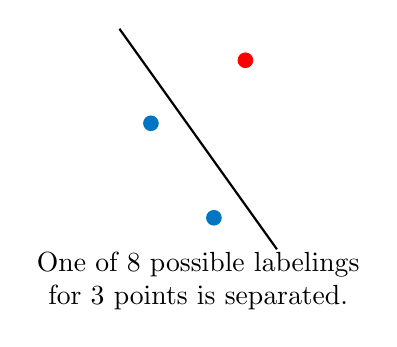
\begin{tikzpicture}[scale=0.8]
			\node[circle, fill=tudelftblue, inner sep=2pt] at (0,1) {};
			\node[circle, fill=red, inner sep=2pt] at (1.5,2) {};
			\node[circle, fill=tudelftblue, inner sep=2pt] at (1,-0.5) {};
			\draw[thick] (-0.5, 2.5) -- (2, -1);
			\node[align=center] at (0.75, -1.5) {One of 8 possible labelings\\for 3 points is separated.};
		\end{tikzpicture}
		\caption{A set of 3 points can be shattered by a line.}
	\end{subfigure}
	\hfill
	\begin{subfigure}{0.48\textwidth}
		\centering
		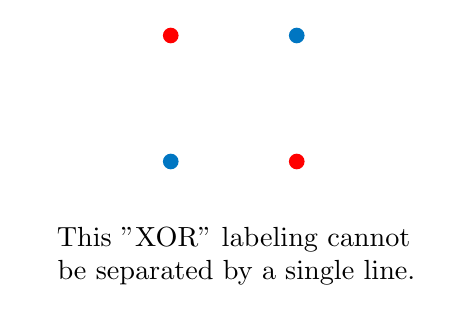
\begin{tikzpicture}[scale=0.8]
			\node[circle, fill=tudelftblue, inner sep=2pt] at (0,0) {};
			\node[circle, fill=tudelftblue, inner sep=2pt] at (2,2) {};
			\node[circle, fill=red, inner sep=2pt] at (0,2) {};
			\node[circle, fill=red, inner sep=2pt] at (2,0) {};
			\node[align=center, text width=5cm] at (1, -1.5) {This "XOR" labeling cannot be separated by a single line.};
		\end{tikzpicture}
		\caption{A set of 4 points cannot be shattered by a line.}
	\end{subfigure}
	\caption{Illustrating the VC-Dimension of a 2D linear classifier, which is 3.}
	\label{fig:vc_dimension}
\end{figure}

\paragraph{Theoretical Importance}
The main value of the VC-dimension is theoretical. It provides a probabilistic upper bound on the true error of a classifier based on its training error and its complexity $h$.  Conceptually, the bound is:
\[ \epsilon \le \epsilon_A + \text{ComplexityPenalty}(h, N, \eta) \]
This confirms our intuition: to keep the generalization error $\epsilon$ close to the training error $\epsilon_A$, we need a classifier with a small VC-dimension $h$.  In practice, these bounds are often too loose to be useful for direct calculation, but they provide the theoretical foundation for why controlling complexity is essential.

\subsection{Controlling Complexity with Support Vector Classifiers}
The \textbf{Support Vector Classifier (SVC)}, or \textbf{Support Vector Machine (SVM)}, is a linear classifier that is explicitly designed to control its complexity and thus generalize well. Instead of finding just \textit{any} hyperplane that separates the data (like the Perceptron), the SVM finds the single, unique, optimal hyperplane that has the \textbf{maximum margin} of separation between the two classes.

\paragraph{The Maximum Margin Principle}
The \textbf{margin} is the distance between the decision boundary and the closest data points from either class. These closest points, which lie on the edge of the margin, are called the \textbf{support vectors}. The intuition is that a larger margin corresponds to a more confident and robust classifier that is less sensitive to small variations in the training data.

Theoretically, maximizing the margin is equivalent to minimizing the classifier's VC-dimension. By finding the simplest possible boundary (in the maximum margin sense), the SVM aims to minimize the gap between the training error and the generalization error.


\paragraph{The Optimization Problem}
Maximizing the margin can be shown to be equivalent to minimizing the squared norm of the weight vector, $||\mathbf{w}||^2$. This leads to a constrained optimization problem, known as the \textbf{hard-margin SVM} formulation (for linearly separable data):
\begin{align}
	\min_{\mathbf{w}, b} \quad & \frac{1}{2} ||\mathbf{w}||^2                                                \\
	\text{subject to} \quad    & y_i(\mathbf{w}^T\mathbf{x}_i + b) \ge 1 \quad \text{for all } i=1, \dots, N
\end{align}
The constraints ensure that all data points are correctly classified and lie outside the margin. The solution to this problem is a decision boundary that depends only on the support vectors, making the model robust and memory-efficient.

\subsection{Non-Linear SVMs: The Kernel Trick}
The true power of Support Vector Machines is their ability to handle non-linearly separable data. This is achieved by combining the idea of feature maps with a clever mathematical shortcut known as the \textbf{Kernel Trick}.

The strategy is as follows:
\begin{enumerate}
	\item Project the original data from its low-dimensional feature space into a much higher-dimensional feature space using a non-linear mapping, $\phi(\mathbf{x})$.
	\item In this higher-dimensional space, the data may now be linearly separable.
	\item Find the maximum-margin linear classifier in this new feature space.
\end{enumerate}
The problem with this approach is that the new feature space can be enormous or even infinite-dimensional, making the computations intractable. This is where the Kernel Trick comes in.

The SVM's optimization problem and its final decision function only ever depend on the inner product (dot product) of feature vectors, not the vectors themselves. The \textbf{Kernel Trick} is to use a \textbf{kernel function}, $K(\mathbf{x}_i, \mathbf{x}_j)$, that computes the inner product of the data points in the high-dimensional space, $\phi(\mathbf{x}_i)^T \phi(\mathbf{x}_j)$, directly from the original low-dimensional vectors.
\begin{equation}
	K(\mathbf{x}_i, \mathbf{x}_j) = \phi(\mathbf{x}_i)^T \phi(\mathbf{x}_j)
\end{equation}
This allows us to get the full benefit of working in a high-dimensional space without ever having to explicitly perform the transformation, which is incredibly efficient.

\paragraph{Popular Kernel Functions}
By simply swapping the standard inner product $ \mathbf{x}_i^T \mathbf{x}_j $ with a kernel function, we can create powerful non-linear SVMs. Two popular kernels are:
\begin{itemize}
	\item \textbf{Polynomial Kernel:} Creates a polynomial decision boundary. The degree of the polynomial, $d$, is a hyperparameter.
	      \begin{equation}
		      K(\mathbf{x}_i, \mathbf{x}_j) = (\mathbf{x}_i^T \mathbf{x}_j + c)^d
	      \end{equation}
	\item \textbf{Radial Basis Function (RBF) Kernel:} A very powerful and popular general-purpose kernel. It can create complex, localized decision boundaries. Its hyperparameter, $\gamma$ (gamma), controls the flexibility of the boundary.
	      \begin{equation}
		      K(\mathbf{x}_i, \mathbf{x}_j) = \exp(-\gamma ||\mathbf{x}_i - \mathbf{x}_j||^2)
	      \end{equation}
\end{itemize}

\subsubsection{Chapter Conclusion}
Understanding \textbf{model complexity} is key to navigating the fundamental \textbf{Bias-Variance Tradeoff}. We saw that complexity is more than just the number of parameters and can be formally characterized by the \textbf{VC-Dimension}. This led us to the \textbf{Support Vector Machine}, a classifier explicitly designed to control complexity by finding a \textbf{maximum margin} solution. Finally, the \textbf{Kernel Trick} allows SVMs to efficiently learn complex, non-linear boundaries, making them one of the most powerful and theoretically elegant classifiers in machine learning.

\section{Regularisation}
\label{sec:ml_regularisation}

This final chapter focuses on \textbf{Regularisation}, a collection of essential techniques designed to combat overfitting. The core idea is to intentionally introduce a preference for simpler models during training, even if it means not fitting the training data as perfectly. As defined by Goodfellow et al., regularization encompasses any technique used to reduce a model's test error, possibly at the expense of an increased training error.

\subsection{The Problem of Overfitting}
As we've seen, a model with high complexity (or "capacity") can easily overfit a limited dataset. It learns not only the underlying signal but also the random noise specific to the training samples. A classic example is polynomial regression: a high-degree polynomial can perfectly pass through every training point but will likely oscillate wildly and perform poorly on new data. Regularisation aims to find a "sweet spot," like the quadratic fit below, that captures the general trend without memorizing the noise.


\subsection{The Regularisation Framework}
The most common way to implement regularisation is by adding a \textbf{penalty term}, $\Omega(\theta)$, to the standard loss function, $J(\theta)$. This creates a new, regularised loss function, $\tilde{J}(\theta)$:
\begin{equation}
	\tilde{J}(\theta) = J(\theta; X, y) + \alpha \Omega(\theta)
	\label{eq:regularisation_framework}
\end{equation}
The components of this framework are:
\begin{itemize}
	\item \textbf{$J(\theta; X, y)$:} The original \textbf{loss term} that measures how well the model with parameters $\theta$ fits the data (e.g., MSE or cross-entropy).
	\item \textbf{$\Omega(\theta)$:} The \textbf{regularisation penalty}. This term measures the complexity of the model. Common choices include penalizing the size of the model's weights.
	\item \textbf{$\alpha$:} The \textbf{regularisation parameter} ($\alpha \ge 0$). This is a hyperparameter that controls the strength of the penalty. It determines the tradeoff between fitting the training data well and keeping the model simple. A larger $\alpha$ encourages a simpler model.
\end{itemize}
During training, the optimizer now minimizes this combined objective. It is forced to find a set of parameters $\theta$ that not only achieves a low data-fitting error but also has low complexity.

\subsection{Parameter Norm Penalties}
This is the most common regularization strategy. It involves adding a penalty term $\Omega(\mathbf{w})$ to the loss function that is a function of the model's weights.

\subsubsection{L2 Regularisation (Weight Decay / Ridge)}
\textbf{L2 Regularisation} adds a penalty proportional to the squared L2 norm of the weight vector, $||\mathbf{w}||_2^2 = \sum_i w_i^2$. This is also known as \textbf{Ridge Regression} in the context of linear models.

The regularised loss function is:
\begin{equation}
	\tilde{J}(\mathbf{w}) = J(\mathbf{w}) + \frac{\alpha}{2} ||\mathbf{w}||_2^2
\end{equation}
This penalty discourages large weight values. During gradient descent, it results in an update rule that effectively shrinks the weights toward zero at each step, which is why it's often called \textbf{weight decay}. It encourages the model to use all features a little bit, rather than relying heavily on just a few.

\subsubsection{L1 Regularisation (Lasso)}
\textbf{L1 Regularisation} adds a penalty proportional to the L1 norm of the weight vector, $||\mathbf{w}||_1 = \sum_i |w_i|$. This is also known as \textbf{Lasso} (Least Absolute Shrinkage and Selection Operator) in linear models.

The regularised loss function is:
\begin{equation}
	\tilde{J}(\mathbf{w}) = J(\mathbf{w}) + \alpha ||\mathbf{w}||_1
\end{equation}
The L1 penalty has a unique and powerful property: it promotes \textbf{sparsity}. As the regularization strength $\alpha$ is increased, many of the model's weights are driven to be exactly zero. This means L1 regularization can be used for \textbf{automatic feature selection}, as it effectively removes irrelevant features from the model, leading to simpler and more interpretable results.



\end{document}
